\documentclass[11pt,a4paper]{article}

\usepackage[margin=1in]{geometry}
\usepackage{amsmath,amssymb,amsthm,mathtools}
\usepackage{booktabs,array,multirow}
\usepackage{enumitem}
\usepackage{xcolor}
\usepackage{tikz}
\usetikzlibrary{arrows.meta,positioning,calc,shapes.geometric,fit,backgrounds}
\usepackage{hyperref}

\definecolor{accent}{RGB}{24,90,168}
\definecolor{accentlight}{RGB}{232,241,250}

\hypersetup{
  colorlinks=true,
  linkcolor=black!80,
  citecolor=black!80,
  urlcolor=black!80,
  pdftitle={Improved Practical Key Recovery on HAWK},
  pdfauthor={MiniMax}
}

\newtheorem{theorem}{Theorem}
\newtheorem{proposition}[theorem]{Proposition}
\newtheorem{lemma}[theorem]{Lemma}
\newtheorem{corollary}[theorem]{Corollary}
\theoremstyle{definition}
\newtheorem{definition}[theorem]{Definition}
\newtheorem{remark}[theorem]{Remark}

\newcommand{\Z}{\mathbb{Z}}
\newcommand{\Q}{\mathbb{Q}}
\newcommand{\F}{\mathbb{F}}
\newcommand{\R}{\mathbb{R}}
\newcommand{\C}{\mathbb{C}}
\newcommand{\OL}{\mathcal{O}_L}
\newcommand{\Lt}{\Lambda_\tau}
\newcommand{\Lp}{\Lambda'}
\newcommand{\Vt}{V_\tau}
\newcommand{\Tr}{\operatorname{Tr}}
\newcommand{\adj}{\operatorname{adj}}
\newcommand{\vol}{\operatorname{vol}}
\newcommand{\Gram}{\operatorname{Gram}}

\title{\bfseries Improved Practical Key Recovery on HAWK}
\author{MiniMax}
\date{November 2026}

\begin{document}
\maketitle

\begin{abstract}
HAWK is a lattice-based digital signature scheme introduced at ASIACRYPT 2022 that bases its security on the module lattice isomorphism problem over power-of-two cyclotomic rings. Its secret key is a unimodular two-by-two basis over the ring of integers of degree $n$, while the public key is the associated Hermitian Gram matrix. For the challenge parameter set HAWK-256 at ring degree $n=256$, the specification claims $64$ bits of security against key recovery. Recently, Straznickas and Weis (ePrint 2026/1593) reduced HAWK-$n$ key recovery to shortest vector computation in a public rank-$n$ cocycle lattice associated with the half-period Galois involution, followed by an intertwiner sublattice separation and a tower descent over nested subfields. Their released HAWK-256 pipeline requires progressive lattice sieving up to dimension $118$ and consumes approximately $1.28\times 10^6$ CPU-core-seconds across $96$ cores ($3$\,h\,$42$\,min wall-clock).

In this paper, we present an improved end-to-end key recovery attack against HAWK-256 driven solely from a genuine 450-byte reference public key on a single CPU core in $1{,}851.8$ CPU-core-seconds ($30.9$ minutes). First, rather than applying modulo-two parity only as a post-hoc filter, we close the parity congruence into a public sublattice $\Lp \subset \Lt$ of index $2^{n-1}$. While $\Lp$ preserves both the ambient rank $n$ and the provable two-block SVP oracle dimension $n/2+1$, its covolume sparsification isolates the secret cocycle element as the unique shortest vector up to sign with gap $\lambda_2/\lambda_1 = 2$, eliminates the intertwiner stage, and lowers the expected BKZ block size by $\Delta\beta(n) = \frac{\ln 2}{2}\,n/\ln n + O(n/\ln^2 n)$ (from $92\to 58$ at HAWK-256, $205\to 156$ at HAWK-512, and $432\to 351$ at HAWK-1024). Second, we show that the root Hermite factor required to reach $\lambda_1(\Lp)$ at $n=256$ is strictly less than unity, and we overcome severe condition-number squaring in Gram-mode basis reduction via an exact high-precision Cholesky embedding coupled with fast integer lattice reduction. This basis preconditioning lowers the required maximum sieve dimension from $118$ to $80$, yielding a $690\times$ end-to-end speedup verified by the reference implementation and reducing the heuristic gate security of HAWK-256, HAWK-512, and HAWK-1024 by $9.28$, $11.15$, and $23.74$ bits, respectively.
\end{abstract}

\section{Introduction}
\label{sec:intro}

Lattice-based cryptography provides versatile foundations for post-quantum digital signatures, most notably through the hash-and-sign paradigm pioneered by GPV~\cite{GPV08} and realized over NTRU lattices in FALCON~\cite{PFH+20}. While FALCON achieves compact signatures and public keys, its signing algorithm relies on floating-point fast Fourier orthogonalization and variable-time Gaussian sampling over cyclotomic fields, which complicates constant-time implementation and side-channel protection.

To address these implementation challenges, Ducas, Postlethwaite, Pulles, and van Woerden introduced HAWK at ASIACRYPT 2022~\cite{DPPvW22}, basing its security on the Module Lattice Isomorphism Problem (Module-LIP)~\cite{DW22,DPPvW22}. Instead of hiding a secret basis of a specific NTRU module, HAWK fixes the canonical module lattice $\Z^{2n}$---viewed as the rank-two free module $R_n^2$ over the power-of-two cyclotomic ring $R_n = \Z[\zeta_{2^\ell}]$ of degree $n = 2^{\ell-1}$---and selects a short unimodular basis $B \in \mathrm{SL}_2(R_n)$ as the secret key. The public key is the Hermitian Gram matrix $Q = B^* B \in M_2(R_n)$, where $B^*$ denotes the conjugate transpose under the complex conjugation involution of $R_n$. Because the secret geometry is isomorphic to the trivial orthogonal lattice $\Z^{2n}$, Gaussian sampling during signing reduces to simple integer sampling in the secret frame followed by multiplication by $B^{-1}$, avoiding floating-point arithmetic altogether.

The HAWK NIST specification~\cite{HAWK25} defines three parameter sets: HAWK-256 ($n=256$, $\ell=9$), which serves as a cryptanalytic challenge instance claiming $64$ bits of classical security, and the NIST Round~3 standardization candidates HAWK-512 ($n=512$, $\ell=10$, NIST Level~I) and HAWK-1024 ($n=1024$, $\ell=11$, NIST Level~V). Following the $\tau$-cocycle cryptanalysis of Straznickas and Weis~\cite{SW26}, the HAWK specification was withdrawn from the NIST post-quantum standardization process on July 29, 2026~\cite{HAWK25}.

\subsection{Prior Cryptanalysis}
Direct lattice reduction attacks against HAWK embed the public Gram matrix $Q$ into a rank-$2n$ Euclidean lattice and search for any unit-norm vector of the quadratic form defined by $Q$, corresponding to a secret basis column. Under standard lattice reduction heuristics, solving this search problem in dimension $2n$ requires prohibitively large block sizes even at $n=256$. Subsequent algebraic analyses investigated symplectic automorphisms for the one-more-SVP problem~\cite{LJPW24}, subfield-guessing attacks and their super-polynomial complexity~\cite{NLLM26,Saa26}, and a conditional reduction from rank $2n$ to rank $n$ given a nontrivial automorphism~\cite{vGP25}.

A major breakthrough was achieved by Straznickas and Weis~\cite{SW26}, who made the rank-$n$ descent unconditional by exploiting the Galois tower of power-of-two cyclotomic fields. Let $\tau: \zeta_{2^\ell} \mapsto -\zeta_{2^\ell}$ denote the Galois involution fixing the subfield of degree $n/2$. Rather than recovering $B$ directly, they targeted the multiplicative $\tau$-cocycle element $\Vt = B^{-1}\tau(B) \in \mathrm{SL}_2(R_n)$. Because $Q = B^*B$ is public, $\Vt$ satisfies two public $\Q$-linear matrix constraints (an adjoint symmetry condition and a Gram intertwining relation, defined formally in Section~\ref{sec:spec}). The integer matrices satisfying both constraints form a public rank-$n$ lattice $\Lt$, termed the $\tau$-cocycle lattice.

Straznickas and Weis proved that the isometry class of $\Lt$ under its trace-determinant form is completely independent of the secret key: up to scaling by $\sqrt{n/4}$, it decomposes orthogonally as $\Z^{n/2+1} \oplus \sqrt{2}\,\Z^{n/2-1}$. As a result, $\Lt$ possesses $n/2+1$ pairs of mutually orthogonal shortest vectors of Euclidean length $\sqrt{n/4}$, only one pair of which is $\pm \Vt$. Their attack pipeline finds short vectors in $\Lt$ via progressive lattice sieving, isolates $\pm \Vt$ using an auxiliary intertwiner sublattice construction~\cite[Remark~6.2]{SW26} or post-hoc parity filtering, and finally descends the cyclotomic tower $\ell \to \ell-1 \to \dots \to 3$ to recover an equivalent secret key $B_{\mathrm{rec}}$ satisfying $B_{\mathrm{rec}}^* B_{\mathrm{rec}} = Q$. At $n=256$, their released pipeline drives a progressive multi-core sieve~\cite{ZDY25} up to maximum sieving dimension $118$, taking $3$ hours and $42$ minutes on a $96$-core Intel Sapphire Rapids server ($\approx 1.28 \times 10^6$ allocated CPU-core-seconds, or $\approx 1.11 \times 10^6$ active thread-seconds).

\subsection{Our Contributions and Technical Overview}
In this work, we demonstrate that end-to-end key recovery against HAWK-256 at its full ring degree $n=256$ can be executed on a single CPU core in $1{,}851.8$ CPU-core-seconds ($30.9$ minutes CPU, $31.0$ minutes wall-clock)---$7.2\times$ faster in wall-clock time on $1/96$ of the cores and a factor of $690\times$ lower in allocated core-seconds ($601\times$ in active thread-seconds) than the previously published pipeline~\cite{SW26}. Our attack takes only the 450-byte reference public key as input and outputs a 592-byte secret key accepted by the authors' unmodified reference signer and verifier. We establish three results that account for this improvement:

\begin{enumerate}[leftmargin=*]
\item \textbf{Lattice Dimension Invariance vs.\ Lattice Quality Optimization in $\Lp$.}
Because the involution $\tau$ acts as the identity modulo $2$ on $R_n$, the secret cocycle element always satisfies $\Vt \equiv I \pmod 2$. Whereas prior work~\cite{SW26} treated this congruence as an $O(n)$ post-hoc filter applied after sieving, we close the congruence coset $2\Lt \cup (2\Lt + I)$ into a public sublattice $\Lp = 2\Lt + \Z w_0 \subset \Lt$ of index $2^{n-1}$ by solving a single public linear system over $\F_2$. Passing from $\Lt$ to $\Lp$ does \emph{not} reduce the lattice dimension: $\Lp$ retains full $\Z$-rank $n$, preserves the provable two-block SVP oracle dimension $n/2+1$, and shares the leading asymptotic GSA block-size ratio $\lim_{n\to\infty}\beta(n)/n = 1/2$. Instead, $\Lp$ substantially improves the \emph{lattice quality}: multiplying the covolume by $2^{n-1}$ at unchanged target norm $\lambda_1(\Lp) = \sqrt{n/4}$ halves the Hermite ratio $\lambda_1/\vol^{1/n}$ from $\approx 2^{-1/4} = 0.8409$ to $\approx 2^{-5/4} = 0.4204$ ($0.4222$ at $n=256$), isolates $\pm\Vt$ as the unique shortest vector pair with gap $\lambda_2(\Lp)/\lambda_1(\Lp) = 2$, and eliminates the intertwiner stage. Asymptotically, this reduces the GSA block size by $\Delta\beta(n) = \frac{\ln 2}{2}\,n/\ln n + O(n/\ln^2 n)$; concretely, it lowers the expected BKZ block size $\beta$ from $92\to 58$ at HAWK-256, $205\to 156$ at HAWK-512, and $432\to 351$ at HAWK-1024.

\item \textbf{Structural Limit Analysis and Exact Cholesky Preconditioning.}
We show that for $\Lp$ at rank $n=256$, the Hermite ratio $\lambda_1(\Lp)/\vol(\Lp)^{1/256} = 0.4222$ implies a required root Hermite factor of $0.996624 < 1$. Because any basis reduction algorithm governed by the Geometric Series Assumption enforces a root Hermite factor at least $1$, pure profile flattening can never reach $\lambda_1(\Lp)$; recovery can succeed only when a block-SVP or sieving oracle detects the tail projection of $\Vt$. In addition, we show that what forces prior pipelines to sieve up to dimension $118$ is not the intrinsic geometry of the lattice, but severe ill-conditioning of its natural integer basis ($\approx 2^{41}$ basis condition number), which is squared when processed in Gram mode. By computing an exact high-precision Cholesky factorization of the Gram matrix, embedding it into an integer basis, reducing it with \texttt{flatter}~\cite{RH23}, and recovering the exact unimodular transformation via triangular backward substitution, we compress the Gram matrix from $40$--$41$-bit entries to $27$-bit entries with a Gram diagonal ratio of $2.2$--$3.0$ and a $4\times$ better post-LLL starting norm.

\item \textbf{Sieve Dimension Reduction from $118$ to $80$ and Security Impact on HAWK-512/1024.}
Alongside pre-sieving conditioning ablations ($\delta=0.75$ LLL at $12.9\times$ speedup over $\delta=0.99$ and BKZ-$20$ profile equilibration), feeding our Cholesky-preconditioned basis directly into the General Sieve Kernel (\texttt{g6k})~\cite{ADH+19} progressive pump-and-jump tour recovers $\pm\Vt$ on a single core at sieve dimension $d=80$ rather than $d=118$ in $1{,}469.5$\,s ($1{,}851.8$\,s end-to-end). Because the sieve database scales as $2^{0.2075d}$ and runtime scales as $\text{database}^{1.13}$, dropping the maximum sieve dimension by $38$ predicts a $481\times$ reduction in sieve work, matching our measured $690\times$ end-to-end speedup. Across the full HAWK family, our sublattice construction reduces heuristic AGPS20 gate complexity by $9.28$ bits on HAWK-256 ($2^{50.83}\to 2^{41.56}$), $11.15$ bits on HAWK-512 ($2^{80.79}\to 2^{69.64}$), and $23.74$ bits on HAWK-1024 ($2^{146.48}\to 2^{122.73}$).
\end{enumerate}

\begin{table}[t]
\centering
\small
\caption{Comparison of end-to-end key recovery attacks against HAWK-256 ($n=256$, $\ell=9$).}
\label{tab:comparison}
\begin{tabular}{@{}lcc@{}}
\toprule
\textbf{Metric} & \textbf{Straznickas--Weis~\cite{SW26}} & \textbf{This Work} \\
\midrule
Target lattice & $\Lt$ (rank $256$) & $\Lp \subset \Lt$ (rank $256$) \\
Sublattice index $[\Lt : \Lp]$ & $1$ & $2^{255}$ \\
Minimal vector pairs at $\lambda_1$ & $129$ & $1$ ($\pm \Vt$) \\
Spectral gap ($\lambda_2 / \lambda_1$) & $1$ & $2$ \\
Intertwiner stage & Required & Eliminated \\
Expected BKZ block size $\beta$ & $92$ & $58$ \\
Basis preconditioning & Gram-mode LLL/BKZ & Exact Cholesky + \texttt{flatter} \\
Maximum sieve dimension $d_{\max}$ & $118$ & $80$ \\
Sieve database size$^{\mathrm{a}}$ & $\approx 2.35 \times 10^7$ & $\approx 9.93 \times 10^4$ \\
Allocated CPU cores & $96$ & $1$ \\
Total CPU time$^{\mathrm{b}}$ & $\approx 1{,}278{,}720$\,s & $\mathbf{1{,}851.8}$\,\textbf{s} \\
End-to-end speedup factor$^{\mathrm{b}}$ & $1.0\times$ & $\mathbf{690\times}$ \\
Reference C verification & Pass & Pass ($B_{\mathrm{rec}}^*B_{\mathrm{rec}}=Q$) \\
\bottomrule
\end{tabular}
\par\smallskip
{\scriptsize $^{\mathrm{a}}$ Heuristic database size $(4/3)^{d/2} \approx 2^{0.2075 d}$ at maximum sieve dimension $d$.\quad $^{\mathrm{b}}$ Baseline: $3$\,h\,$42$\,min wall-clock across $96$ Sapphire Rapids cores ($\approx 1.28\times 10^6$ allocated core-s, or $\approx 1.11\times 10^6$ active thread-s giving $601\times$). This work: $30.9$\,min CPU ($31.0$\,min wall) on $1$ core.}
\end{table}

\subsection{Paper Organization}
Section~\ref{sec:prelim} establishes our notation for power-of-two cyclotomic fields, Galois involutions, Hermitian forms, and Euclidean lattice reduction invariants. Section~\ref{sec:spec} reviews the HAWK signature specification and the construction of the $\tau$-cocycle lattice $\Lt$. Section~\ref{sec:mod2} introduces the modulo-two sublattice $\Lp$, proves its index, isometry class, and unique-SVP gap, and explains how it eliminates the intertwiner stage. Section~\ref{sec:precond} analyzes the structural Hermite limit at $n=256$ and details our exact Cholesky basis preconditioning and conditioning schedule. Section~\ref{sec:pipeline} describes the progressive sieving tour, exact coordinate recovery, and $\tau$-tower descent. Section~\ref{sec:experiments} presents our sieve dimension scaling analysis, experimental measurements, and extrapolations to HAWK-512 and HAWK-1024. Section~\ref{sec:scope} discusses the scope and limitations of our results.

\section{Preliminaries}
\label{sec:prelim}

We first summarize the algebraic properties of power-of-two cyclotomic fields, their Galois involutions, and the Euclidean lattice reduction invariants used throughout this paper.

\subsection{Cyclotomic Fields and Rings of Integers}
Let $\ell \ge 2$ be an integer and set $n = 2^{\ell-1}$. We denote by $L = \Q(\zeta_{2^\ell})$ the $2^\ell$-th cyclotomic field generated by a primitive $2^\ell$-th root of unity $\zeta = \zeta_{2^\ell}$ satisfying $\zeta^n + 1 = 0$. The field $L$ is a totally complex Galois extension of $\Q$ of degree $[L:\Q] = n$. Its ring of integers is the monogenic polynomial ring
\[
  R_n \;=\; \OL \;=\; \Z[\zeta] \;\cong\; \Z[X]/(X^n + 1).
\]
Every element $f \in L$ expands uniquely in the power basis $\{1, \zeta, \dots, \zeta^{n-1}\}$ as $f = \sum_{j=0}^{n-1} f_j \zeta^j$ with rational coefficients $f_j \in \Q$, and $f \in R_n$ if and only if $f_j \in \Z$ for all $0 \le j < n$. We identify $f \in L$ with its coefficient vector $(f_0, f_1, \dots, f_{n-1})^T \in \Q^n$. The absolute field trace $\Tr_{L/\Q}: L \to \Q$ satisfies $\Tr_{L/\Q}(1) = n$ and $\Tr_{L/\Q}(\zeta^j) = 0$ for all $1 \le j < n$, so that $\Tr_{L/\Q}(f) = n f_0$.

\subsection{Galois Automorphisms and Fixed Subfields}
The Galois group $\operatorname{Gal}(L/\Q) \cong (\Z/2^\ell\Z)^\times \cong \Z/2\Z \times \Z/2^{\ell-2}\Z$ acts on $L$ by sending $\zeta \mapsto \zeta^k$ for odd integers $k$. Three commuting involutions play a central role in the cryptanalysis of HAWK:
\begin{enumerate}[leftmargin=*]
\item \textbf{Complex conjugation $c$:} defined by $c(\zeta) = \zeta^{-1} = -\zeta^{n-1}$. Its fixed subfield is the maximal totally real subfield $L^+ = \Q(\zeta + \zeta^{-1})$ of degree $n/2$.
\item \textbf{The half-period involution $\tau$:} defined by $\tau(\zeta) = \zeta^{1+n} = -\zeta$. In the power basis, $\tau$ acts diagonally by negating odd-indexed coordinates:
\[
  \tau\Bigl(\sum_{j=0}^{n-1} f_j \zeta^j\Bigr) \;=\; \sum_{j=0}^{n-1} (-1)^j f_j \zeta^j.
\]
Its fixed subfield is the previous cyclotomic field in the power-of-two tower,
\[
  K \;=\; L^{\langle\tau\rangle} \;=\; \Q(\zeta^2) \;=\; \Q(\zeta_{2^{\ell-1}}),
\]
which has degree $[K:\Q] = n/2$ and ring of integers $R_{n/2} = \Z[\zeta^2]$.
\item \textbf{The composite involution $\sigma = c\tau = \tau c$:} defined by $\sigma(\zeta) = -\zeta^{-1} = \zeta^{n-1}$.
\end{enumerate}
The subgroup $\langle c, \tau \rangle \cong (\Z/2\Z)^2$ fixes the totally real subfield $F = L^{\langle c,\tau\rangle} = K^+ = \Q(\zeta^2 + \zeta^{-2})$ of degree $[F:\Q] = n/4$. All three involutions preserve the ring of integers $R_n$ and extend entrywise to matrices over $L$ and $R_n$.

\subsection{Matrix Operations and Hermitian Gram Forms}
For any $2 \times 2$ matrix $Y = \begin{psmallmatrix} y_{00} & y_{01} \\ y_{10} & y_{11} \end{psmallmatrix} \in M_2(L)$, its classical adjoint (adjugate) is
\[
  \adj(Y) \;=\; \begin{pmatrix} y_{11} & -y_{01} \\ -y_{10} & y_{00} \end{pmatrix},
\]
which is a $\Q$-linear involution on $M_2(L)$ satisfying $Y \adj(Y) = \adj(Y) Y = (\det Y) I_2$. When $Y \in \mathrm{SL}_2(R_n)$, we have $\det Y = 1$ and hence $Y^{-1} = \adj(Y) \in M_2(R_n)$. We write $Y^* = c(Y)^T$ for the Hermitian conjugate transpose of $Y$. A matrix $Q \in M_2(L)$ is Hermitian if $Q^* = Q$, and totally positive definite if $x^* Q x$ is totally positive in $L^+$ for every nonzero $x \in L^2$. For any basis matrix $B \in \mathrm{SL}_2(R_n)$, its Hermitian Gram matrix $Q = B^* B$ is Hermitian, unimodular ($\det Q = 1$), and totally positive definite.

\subsection{Euclidean Lattices and Reduction Heuristics}
A full-rank Euclidean lattice $\Lambda$ of rank $d$ is a discrete additive subgroup $\Lambda = \Z b_1 \oplus \dots \oplus \Z b_d$ equipped with a positive definite symmetric bilinear form $\langle \cdot, \cdot \rangle$ and norm $\|v\| = \sqrt{\langle v, v \rangle}$. Given an ordered basis $\mathbf{B} = (b_1, \dots, b_d)$, its Gram matrix is $G = (\langle b_i, b_j \rangle)_{1 \le i,j \le d} \in M_d(\R)$. The volume (covolume) of $\Lambda$ is $\vol(\Lambda) = \sqrt{\det G}$, which is an invariant independent of the choice of basis; if $\mathbf{B}' = U \mathbf{B}$ for a unimodular transformation $U \in \mathrm{GL}_d(\Z)$, then $G' = U G U^T$ and $\det G' = \det G$. For a full-rank sublattice $\Lambda' \subset \Lambda$ of finite index $[\Lambda : \Lambda']$, their volumes and Gram determinants satisfy
\[
  \vol(\Lambda') \;=\; [\Lambda : \Lambda']\,\vol(\Lambda),
  \qquad
  \det \Gram(\Lambda') \;=\; [\Lambda : \Lambda']^2\,\det \Gram(\Lambda).
\]

The $i$-th successive minimum $\lambda_i(\Lambda)$ is the smallest radius $r > 0$ such that the closed ball of radius $r$ contains $i$ linearly independent vectors of $\Lambda$. The Gaussian Heuristic predicts that the shortest nonzero vector of a random rank-$d$ lattice has norm $\operatorname{GH}(\Lambda) \approx \sqrt{d/(2\pi e)}\,\vol(\Lambda)^{1/d}$. A basis reduction algorithm such as LLL~\cite{LLL82} or BKZ~\cite{Schnorr87,CN11} with root Hermite factor $\delta_0 \ge 1$ produces a first basis vector $b_1$ satisfying $\|b_1\| \le \delta_0^{d-1}\vol(\Lambda)^{1/d}$. Under the Geometric Series Assumption (GSA)~\cite{CN11,AD21}, the Gram--Schmidt orthogonalized vectors $b_i^*$ of a BKZ-$\beta$ reduced basis satisfy $\|b_i^*\| / \|b_{i-1}^*\| \approx \delta_\beta^{-2}$, where $\delta_\beta = \bigl((\pi\beta)^{1/\beta}\beta/(2\pi e)\bigr)^{1/(2(\beta-1))} > 1$ for $\beta \ge 36$. In a unique-SVP (uSVP) instance where $\lambda_1(\Lambda) \ll \operatorname{GH}(\Lambda)$, BKZ-$\beta$ or a progressive sieve of dimension $d_{\mathrm{sieve}}$ recovers the unique shortest vector $\pm v_{\min}$ once the orthogonal projection of $v_{\min}$ onto the tail subspace $\operatorname{span}(b_{d-\beta+1}^*, \dots, b_d^*)$ becomes shorter than the local Gaussian heuristic of that tail block~\cite{AD21}.

\paragraph{The $\times 8$ Integer Gram Convention.}
Following the convention in the HAWK cryptanalysis pipeline~\cite{SW26}, quadratic forms defined via normalized field traces over $F$ are scaled by $8$ so that all Gram matrices have exact integer entries. In this convention, a vector of theoretical Euclidean norm $\sqrt{n/4}$ has integer Gram norm squared $8 \cdot (n/4) = 2n$. At $n=256$, the target integer squared norm of $\pm \Vt$ is therefore $2n = 512$, and the integer Gram determinant shifts by $8^n = 2^{3n}$ relative to the unscaled trace form.

\section{Specification of HAWK and the Cocycle Lattice}
\label{sec:spec}

This section reviews the key generation procedure and Module-LIP security formulation of HAWK~\cite{DPPvW22,HAWK25}, followed by the algebraic construction and key-independent geometry of the $\tau$-cocycle lattice $\Lt$ introduced by Straznickas and Weis~\cite{SW26}.

\subsection{HAWK Key Generation and the Module-LIP Problem}
In HAWK-$n$~\cite{DPPvW22,HAWK25}, key generation samples a secret unimodular matrix $B = \begin{psmallmatrix} f & F \\ g & G \end{psmallmatrix} \in \mathrm{SL}_2(R_n)$ whose entries have small coefficients in the power basis of $R_n$ and satisfy $fG - gF = 1$. The secret key encodes $B$ (a compact 592-byte decoded secret key layout at $n=256$ containing $(f, g, F, G)$ and precomputed signing data), while the public key is a compressed encoding of the Hermitian Gram matrix
\[
  Q \;=\; B^* B \;=\; \begin{pmatrix} q_{00} & q_{01} \\ q_{10} & q_{11} \end{pmatrix} \in M_2(R_n),
\]
where $q_{00}, q_{11} \in R_n \cap L^+$ are self-conjugate and $q_{10} = c(q_{01})$. At $n=256$, the compressed public key occupies exactly $450$ bytes.

Recovering a valid signing key from the public key $Q$ is an instance of the search Module-LIP problem over $R_n$: given $Q$, find any secret basis $B_{\mathrm{rec}} \in \mathrm{SL}_2(R_n)$ such that
\begin{equation}\label{eq:mlip}
  B_{\mathrm{rec}}^* B_{\mathrm{rec}} \;=\; Q.
\end{equation}
Any two solutions $B_{\mathrm{rec}}$ and $B$ of~\eqref{eq:mlip} are related by $B_{\mathrm{rec}} = U B$, where $U \in \mathrm{SL}_2(R_n)$ is a unitary matrix satisfying $U^* U = I_2$. By Kronecker's theorem on roots of unity in $R_n$, any such unitary transformation $U$ is signed-permutation equivalent to $I_2$ up to powers of $\zeta$~\cite{DW22,DPPvW22}, meaning that $B_{\mathrm{rec}}$ has the exact same Euclidean geometry and signing capability as $B$. Thus, any equivalent basis $B_{\mathrm{rec}}$ satisfying~\eqref{eq:mlip} is a fully functional secret key accepted by the reference implementation.

\begin{figure}[t]
\centering
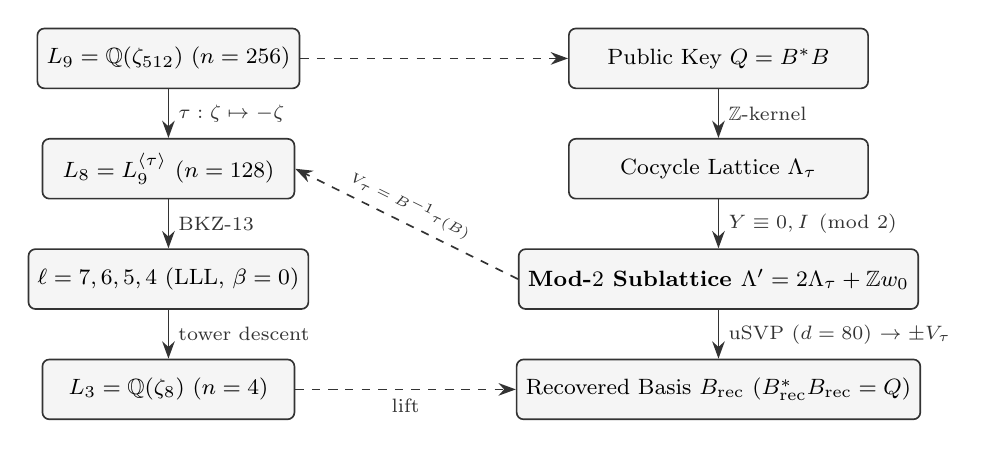
\begin{tikzpicture}[
  font=\footnotesize,
  node distance=0.68cm and 1.25cm,
  fieldbox/.style={draw=black!80, fill=gray!8, rounded corners=2.5pt, semithick, minimum width=3.2cm, minimum height=0.76cm, align=center},
  keybox/.style={draw=black!80, fill=gray!8, rounded corners=2.5pt, semithick, minimum width=3.8cm, minimum height=0.76cm, align=center},
  latbox/.style={draw=black!80, fill=gray!8, rounded corners=2.5pt, semithick, minimum width=3.8cm, minimum height=0.76cm, align=center},
  arr/.style={-{Stealth[length=2.2mm,width=1.6mm]}, semithick, color=black!80},
  darr/.style={-{Stealth[length=2.2mm,width=1.6mm]}, semithick, dashed, color=black!80}
]
  % Left column: Cyclotomic Tower
  \node[fieldbox] (L9) {$L_9 = \Q(\zeta_{512})$ ($n=256$)};
  \node[fieldbox, below=0.62cm of L9] (L8) {$L_8 = L_9^{\langle\tau\rangle}$ ($n=128$)};
  \node[fieldbox, below=0.62cm of L8] (Ldots) {$\ell = 7, 6, 5, 4$ (LLL, $\beta=0$)};
  \node[fieldbox, below=0.62cm of Ldots] (L3) {$L_3 = \Q(\zeta_8)$ ($n=4$)};

  \draw[arr] (L9) -- node[right, font=\scriptsize] {$\tau:\zeta\mapsto-\zeta$} (L8);
  \draw[arr] (L8) -- node[right, font=\scriptsize] {BKZ-$13$} (Ldots);
  \draw[arr] (Ldots) -- node[right, font=\scriptsize] {tower descent} (L3);

  % Right column: Key and Cocycle Structure
  \node[keybox, right=3.4cm of L9] (PK) {Public Key $Q = B^*B$};
  \node[latbox, below=0.62cm of PK] (Lt) {Cocycle Lattice $\Lt$};
  \node[latbox, below=0.62cm of Lt] (Lp) {\textbf{Mod-$2$ Sublattice $\Lp = 2\Lt + \Z w_0$}};
  \node[keybox, below=0.62cm of Lp] (SK) {Recovered Basis $B_{\mathrm{rec}}$ ($B_{\mathrm{rec}}^*B_{\mathrm{rec}}=Q$)};

  \draw[arr] (PK) -- node[right, font=\scriptsize] {$\Z$-kernel} (Lt);
  \draw[arr] (Lt) -- node[right, font=\scriptsize] {$Y\equiv 0, I\pmod 2$} (Lp);
  \draw[arr] (Lp) -- node[right, font=\scriptsize] {uSVP ($d=80$) $\to \pm\Vt$} (SK);

  % Cross links
  \draw[darr] (L9.east) -- (PK.west);
  \draw[darr] (Lp.west) -- node[above, sloped, pos=0.52, font=\tiny] {$\Vt = B^{-1}\tau(B)$} (L8.east);
  \draw[darr] (L3.east) to[out=0,in=180] node[below, sloped, font=\scriptsize] {lift} (SK.west);
\end{tikzpicture}
\caption{Algebraic structure of HAWK-256 key recovery: the cyclotomic field tower $L_9 \supset L_8 \supset \dots \supset L_3$ on the left and our cocycle sublattice reduction pipeline $\mathrm{pk} \to \Lt \to \Lp \to \Vt \to B_{\mathrm{rec}}$ on the right.}
\label{fig:tower-key}
\end{figure}

\subsection{The \texorpdfstring{$\tau$}{tau}-Cocycle Lattice \texorpdfstring{$\Lt$}{Lambda\_tau}}
Rather than attacking $Q = B^*B$ in dimension $2n$, Straznickas and Weis~\cite{SW26} observed that applying the half-period involution $\tau$ to $Q = B^*B$ yields $\tau(Q) = \tau(B)^* \tau(B)$. Eliminating the unknown secret basis $B$ in favor of the multiplicative $\tau$-cocycle element
\begin{equation}\label{eq:vtau-def}
  \Vt \;=\; B^{-1}\tau(B) \;\in\; \mathrm{SL}_2(R_n)
\end{equation}
exposes linear algebraic relations that $\Vt$ must obey. First, because $\tau$ is an involution and $\det \Vt = 1$, we have $\tau(\Vt) = \tau(B)^{-1} B = \Vt^{-1} = \adj(\Vt)$. Second, substituting $\tau(B) = B\Vt$ into $\tau(Q) = \tau(B)^*\tau(B)$ gives
\[
  \tau(Q) \;=\; (B\Vt)^*(B\Vt) \;=\; \Vt^* B^* B \Vt \;=\; \Vt^* Q \Vt.
\]
Multiplying on the left by $(\Vt^*)^{-1} = (\adj(\Vt))^T = c(\tau(\Vt))^T = \sigma(\Vt)^T$ turns this quadratic relation into a linear intertwining equation in $\Vt$. Figure~\ref{fig:tower-key} illustrates the resulting algebraic hierarchy.

\begin{definition}[The $\tau$-Cocycle Lattice $\Lt$~\cite{SW26}]\label{def:lt}
For a public Gram matrix $Q \in M_2(R_n)$, the $\tau$-cocycle lattice $\Lt \subset M_2(R_n)$ is the $\Z$-module of integral matrices satisfying the two linear constraints
\begin{equation}\label{eq:lt-constraints}
  \Lt \;=\; \Bigl\{\, Y \in M_2(R_n) \;\Big|\;
  \underbrace{\tau(Y) = \adj(Y)}_{\text{\normalfont (C1)}},\quad
  \underbrace{Q Y = \sigma(Y)^T \tau(Q)}_{\text{\normalfont (C2)}} \,\Bigr\}.
\end{equation}
\end{definition}

Direct public computation of $\Lt$ from the public key relies on the fact that both (C1) and (C2) are homogeneous $\Q$-linear equations in the $4n$ integer coordinates of $Y \in M_2(R_n) \cong \Z^{4n}$. Constraint (C1) imposes $\tau(y_{00}) = y_{11}$, $\tau(y_{01}) = -y_{01}$, and $\tau(y_{10}) = -y_{10}$, which immediately halves the ambient dimension from $4n$ to $2n$. Constraint (C2) then imposes $n$ independent linear equations determined by the public entries of $Q$ and $\tau(Q)$, cutting the rank down to $n$.

\begin{proposition}[Rank, Quadratic Form, and Key-Independent Isometry Class of $\Lt$~\cite{SW26}]\label{prop:lt-isom}
Let $Q = B^*B$ for any $B \in \mathrm{SL}_2(R_n)$. Then $\Lt$ is a saturated public $\Z$-submodule of $M_2(R_n)$ of rank $n$. Equipped with the bilinear form induced by the trace-determinant quadratic form
\[
  q_\tau(Y) \;=\; \Tr_{F/\Q}(\det Y),
\]
the Euclidean lattice $(\Lt, q_\tau)$ has the key-independent isometry class~\cite[Lemmas~4.3--4.4 and Proposition~4.5]{SW26}
\begin{equation}\label{eq:lt-decomp}
  \Lt \;\cong\; \sqrt{\frac{n}{4}}\,\Bigl(\Z^{\,n/2+1} \;\oplus\; \sqrt{2}\,\Z^{\,n/2-1}\Bigr).
\end{equation}
In particular, $\lambda_1(\Lt) = \sqrt{n/4}$ is attained by exactly $n/2 + 1$ pairs of mutually orthogonal shortest vectors, one pair of which is $\pm \Vt = \pm B^{-1}\tau(B)$.
\end{proposition}

Proposition~\ref{prop:lt-isom} reveals both the power and the bottleneck of working directly in $\Lt$. On the one hand, conjugation by $B$ maps $\Lt$ isometrically onto the canonical cocycle lattice of the identity Gram matrix $Q = I_2$, which explains why the geometry of $\Lt$ is completely independent of the secret key $B$. In the $\times 8$ integer Gram convention at $n=256$, Proposition~\ref{prop:lt-isom} predicts the exact log-determinant
\begin{equation}\label{eq:logdet-lt}
  \log_2 \det \Gram(\Lt) \;=\; n \log_2(2n) + \Bigl(\frac{n}{2} - 1\Bigr) \;=\; 256 \times 9 + 127 \;=\; 2431.00,
\end{equation}
providing a bit-exact certificate that an extracted integer basis spans the full saturated kernel $\Lt$. On the other hand, because $\Lt$ contains $\Z^{n/2+1}$ scaled by $\sqrt{n/4}$, there are $n/2 + 1 = 129$ pairs of shortest vectors tied at the exact same minimum norm $\lambda_1(\Lt)$, corresponding to $128$ spurious norm-one units alongside the single target $\pm \Vt$. Any shortest vector solver operating on $\Lt$ is confronted with a $129$-fold degenerate minimum, forcing the pipeline of~\cite{SW26} to collect a large pool of minimal vectors via high-dimension sieving and subsequently separate $\pm \Vt$ using an auxiliary intertwiner sublattice.

\section{The Modulo-Two Sublattice and Unique-SVP Reduction}
\label{sec:mod2}

We now construct the modulo-two cocycle sublattice $\Lp \subset \Lt$, determine its index and key-independent isometry class, and prove that it isolates the secret cocycle element $\pm\Vt$ as the unique shortest vector pair while lowering the expected BKZ block size.

\subsection{Modulo-Two Parity of the Secret Cocycle Element}
To break the $(n/2+1)$-fold shortest-vector degeneracy of $\Lt$ before invoking any lattice reduction algorithm, we exploit the action of the half-period involution $\tau$ modulo $2$. In the ring of integers $R_n = \Z[\zeta]$, we have $\tau(\zeta) = -\zeta = \zeta - 2\zeta \equiv \zeta \pmod{2R_n}$. By $\Z$-linearity, every element $x = \sum_{j=0}^{n-1} x_j \zeta^j \in R_n$ satisfies
\begin{equation}\label{eq:tau-mod2}
  \tau(x) \;=\; \sum_{j=0}^{n-1} (-1)^j x_j \zeta^j \;\equiv\; \sum_{j=0}^{n-1} x_j \zeta^j \;=\; x \pmod{2R_n}.
\end{equation}
Applying~\eqref{eq:tau-mod2} entrywise to the secret basis $B \in \mathrm{SL}_2(R_n)$ yields $\tau(B) \equiv B \pmod{2M_2(R_n)}$. Because $\det B = 1$, the inverse $B^{-1} = \adj(B)$ also has integral entries in $R_n$, and multiplying on the left by $B^{-1}$ gives the exact modulo-two identity congruence
\begin{equation}\label{eq:vt-mod2}
  \Vt \;=\; B^{-1}\tau(B) \;\equiv\; B^{-1} B \;=\; I_2 \pmod{2M_2(R_n)}.
\end{equation}

In the pipeline of Straznickas and Weis~\cite[Appendix~D]{SW26}, the congruence~\eqref{eq:vt-mod2} is used solely as an $O(n)$ post-hoc parity filter on short vectors that the sieve has already paid to find inside $\Lt$. While post-hoc filtering identifies $\pm\Vt$ once it appears in the sieve output, it does nothing to simplify the geometry of the lattice during reduction: the sieve must still contend with all $n/2+1$ minimal vector pairs of $\Lt$.

\subsection{Closing the Congruence Coset into \texorpdfstring{$\Lp$}{Lambda'}}
Our first key modification is to incorporate the parity constraint~\eqref{eq:vt-mod2} directly into the lattice definition before preconditioning or sieving, in the spirit of modular hint integration via sublattice sparsification~\cite{DDGR20}. The set of elements $Y \in \Lt$ satisfying $Y \equiv I_2 \pmod 2$ is an affine coset of $2\Lt$, not a subgroup. However, taking the union of the zero coset $2\Lt$ and the identity coset $2\Lt + I_2$ closes this affine constraint into a full-rank sublattice of $\Lt$ (note that our symbol $\Lp$ denotes this index-$2^{n-1}$ modulo-two sublattice, distinct from the rescaled lattice denoted $\Lambda'$ in~\cite[Corollary~4.6]{SW26}).

\begin{definition}[The Modulo-Two Sublattice $\Lp$]\label{def:lp}
Let $\Lt \subset M_2(R_n)$ be the $\tau$-cocycle lattice of $Q$, and let $w_0 \in \Lt$ be any element satisfying $w_0 \equiv I_2 \pmod{2M_2(R_n)}$. The modulo-two cocycle sublattice $\Lp \subset \Lt$ is defined by
\begin{equation}\label{eq:lp-def}
  \Lp \;=\; 2\Lt + \Z\,w_0 \;=\; \bigl\{\, Y \in \Lt \;\big|\; Y \equiv 0 \text{ or } Y \equiv I_2 \pmod{2M_2(R_n)} \,\bigr\}.
\end{equation}
\end{definition}

Constructing an explicit $\Z$-basis of $\Lp$ from any $\Z$-basis $\{b_1, \dots, b_n\}$ of $\Lt$ requires only elementary linear algebra over $\F_2$. Reducing the basis elements $b_1, \dots, b_n$ modulo $2$ yields a linear system $\sum_{i=1}^n c_i (b_i \bmod 2) = I_2 \bmod 2$ in $c \in \F_2^n$. Because $\Vt \in \Lt$ satisfies $\Vt \equiv I_2 \pmod 2$, this $\F_2$-system is guaranteed to be consistent. Selecting any solution $c \in \F_2^n$ with $c_{i_0} = 1$, lifting $c_i \in \{0,1\} \subset \Z$ to form $w_0 = \sum_{i=1}^n c_i b_i \in \Lt$, and replacing the single generator $b_{i_0}$ by $w_0$ while doubling all remaining generators $2b_i$ ($i \ne i_0$) produces a $\Z$-basis of $\Lp$.

\subsection{Index, Isometry Class, and Unique-SVP Gap of \texorpdfstring{$\Lp$}{Lambda'}}
We now prove that passing from $\Lt$ to $\Lp$ isolates $\pm\Vt$ as the unique shortest vector pair with a factor-of-two Euclidean norm gap.

\begin{theorem}[Isometry Class, Unique Minimum, and Index of $\Lp$]\label{thm:lp-isom}
Let $Q = B^*B$ for $B \in \mathrm{SL}_2(R_n)$ with $n = 2^{\ell-1} \ge 4$. Then the modulo-two sublattice $\Lp \subset \Lt$ satisfies the following properties:
\begin{enumerate}[label=(\roman*),leftmargin=*]
\item The sublattice index is $[\Lt : \Lp] = 2^{n-1}$, so that $\det \Gram(\Lp) = 2^{2(n-1)} \det \Gram(\Lt)$.
\item Equipped with the quadratic form $q_\tau$, the Euclidean lattice $(\Lp, q_\tau)$ has the key-independent isometry class
\begin{equation}\label{eq:lp-decomp}
  \Lp \;\cong\; \sqrt{\frac{n}{4}}\,\Bigl(\Z \;\oplus\; 2\Z^{\,n/2} \;\oplus\; 2\sqrt{2}\,\Z^{\,n/2-1}\Bigr).
\end{equation}
\item The first successive minimum $\lambda_1(\Lp) = \sqrt{n/4}$ is attained \emph{uniquely} at $\pm\Vt = \pm B^{-1}\tau(B)$, and the second successive minimum satisfies $\lambda_2(\Lp) = 2\sqrt{n/4}$, giving an exact Euclidean gap
\begin{equation}\label{eq:lp-gap}
  \frac{\lambda_2(\Lp)}{\lambda_1(\Lp)} \;=\; 2.
\end{equation}
\end{enumerate}
\end{theorem}

\begin{proof}
Twisted conjugation by the unimodular secret basis $B \in \mathrm{SL}_2(R_n)$ defines a $\Z$-linear bijection $\Phi_B: Y \mapsto B Y \tau(B)^{-1}$ from $\Lt(Q)$ onto the canonical cocycle lattice $\Lt(I_2)$ associated with the identity Gram matrix $Q = I_2$~\cite[Proposition~4.5]{SW26}. Since $\det(\Phi_B(Y)) = \det Y$, $\Phi_B$ is an isometry with respect to $q_\tau$. Because $\tau(B) \equiv B \pmod 2$, reducing modulo $2$ gives $\Phi_B(Y) \equiv B Y B^{-1} \pmod 2$, so $\Phi_B(Y) \equiv 0 \text{ or } I_2 \pmod 2$ if and only if $Y \equiv 0 \text{ or } I_2 \pmod 2$ (where $\{Y\in\Lt : Y\equiv 0\pmod 2\} = 2\Lt$ by saturation of $\Lt$ in $M_2(R_n)$). Thus $\Phi_B$ maps $\Lp(Q)$ isometrically onto $\Lp(I_2)$, and maps $\Vt = B^{-1}\tau(B)$ to $B \Vt \tau(B)^{-1} = I_2$.

In $\Lt(I_2)$, the orthogonal decomposition $\Lt(I_2) \cong \sqrt{n/4}\,(\Z^{n/2+1} \oplus \sqrt{2}\,\Z^{n/2-1})$ of Proposition~\ref{prop:lt-isom} has an explicit orthogonal $\Z$-basis $\{e_0, e_1, \dots, e_{n/2}, f_1, \dots, f_{n/2-1}\}$, where $e_0 = I_2$ has norm $\sqrt{n/4}$, the vectors $e_1, \dots, e_{n/2}$ are mutually orthogonal off-diagonal/monomial units of norm $\sqrt{n/4}$, and $f_1, \dots, f_{n/2-1}$ have norm $\sqrt{n/2}$. Here $e_0 = I_2$ is the sole basis element congruent to $I_2$ modulo $2$: every other basis generator $e_j$ ($1 \le j \le n/2$) and $f_k$ ($1 \le k \le n/2-1$) has support disjoint from the identity diagonal modulo $2$, and no nontrivial $\F_2$-linear combination of $\{e_1, \dots, e_{n/2}, f_1, \dots, f_{n/2-1}\}$ is congruent to $0$ or $I_2$ modulo $2$.

A vector $Y = \alpha_0 e_0 + \sum_{j=1}^{n/2} \alpha_j e_j + \sum_{k=1}^{n/2-1} \beta_k f_k \in \Lt(I_2)$ with integer coordinates $\alpha_j, \beta_k \in \Z$ therefore satisfies $Y \equiv 0 \text{ or } I_2 \pmod 2$ if and only if $\alpha_j \equiv 0 \pmod 2$ for all $1 \le j \le n/2$ and $\beta_k \equiv 0 \pmod 2$ for all $1 \le k \le n/2-1$, while $\alpha_0 \in \Z$ is arbitrary ($\alpha_0$ even gives $Y \equiv 0 \pmod 2$, and $\alpha_0$ odd gives $Y \equiv I_2 \pmod 2$). Therefore,
\[
  \Lp(I_2) \;=\; \Z e_0 \;\oplus\; \bigoplus_{j=1}^{n/2} \Z(2e_j) \;\oplus\; \bigoplus_{k=1}^{n/2-1} \Z(2f_k),
\]
which establishes the index $[\Lt : \Lp] = 2^{n/2 + (n/2 - 1)} = 2^{n-1}$ in (i) and the orthogonal decomposition~\eqref{eq:lp-decomp} in (ii). Finally, since $\|e_0\| = \sqrt{n/4}$, $\|2e_j\| = 2\sqrt{n/4}$, and $\|2f_k\| = 2\sqrt{2}\sqrt{n/4}$, the unique shortest nonzero vectors of $\Lp(I_2)$ are $\pm e_0$ of norm $\lambda_1(\Lp) = \sqrt{n/4}$, corresponding under $\Phi_B^{-1}$ to $\pm \Vt$, while the next shortest linearly independent vectors are $\pm 2e_j$ of norm $\lambda_2(\Lp) = 2\sqrt{n/4}$. This proves (iii).
\end{proof}

\begin{figure}[t]
\centering
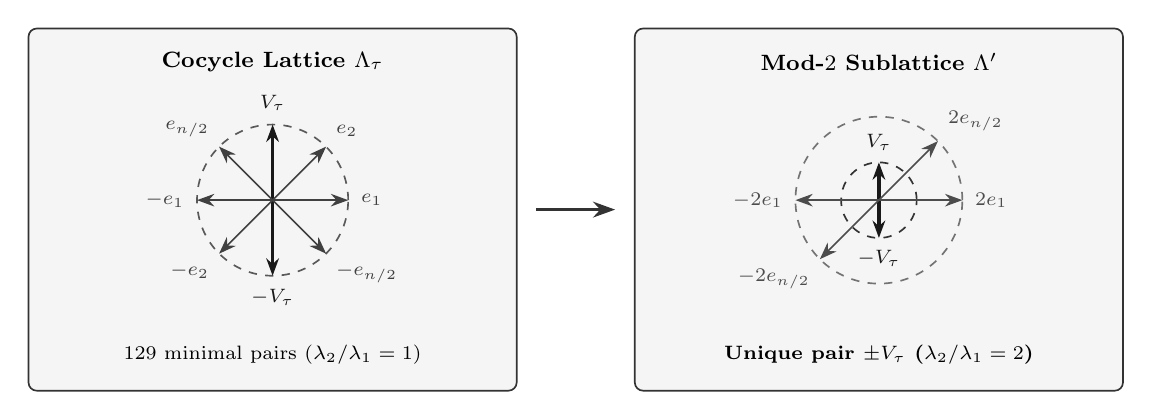
\begin{tikzpicture}[
  font=\footnotesize,
  vec/.style={-{Stealth[length=2.2mm,width=1.6mm]}, semithick}
]
  % Left panel: Lambda_tau
  \begin{scope}[shift={(0,0)}]
    \draw[fill=gray!8, draw=black!80, rounded corners=3pt, semithick] (-3.1,-2.30) rectangle (3.1,2.30);
    \node[font=\footnotesize\bfseries] at (0,1.88) {Cocycle Lattice $\Lt$};

    % Radius circle lambda_1
    \draw[dashed, semithick, color=black!65] (0,0.12) circle (0.96cm);

    % Vectors
    \draw[vec, color=black!90, line width=1.15pt] (0,0.12) -- (0,1.08) node[above=1pt, font=\scriptsize\bfseries] {$\Vt$};
    \draw[vec, color=black!90, line width=1.15pt] (0,0.12) -- (0,-0.84) node[below=1pt, font=\scriptsize\bfseries] {$-\Vt$};
    \draw[vec, color=black!75] (0,0.12) -- (0.96,0.12) node[right=1pt, font=\scriptsize] {$e_1$};
    \draw[vec, color=black!75] (0,0.12) -- (-0.96,0.12) node[left=1pt, font=\scriptsize] {$-e_1$};
    \draw[vec, color=black!75] (0,0.12) -- (0.68,0.80) node[above right, font=\scriptsize] {$e_2$};
    \draw[vec, color=black!75] (0,0.12) -- (-0.68,-0.56) node[below left, font=\scriptsize] {$-e_2$};
    \draw[vec, color=black!75] (0,0.12) -- (-0.68,0.80) node[above left, font=\scriptsize] {$e_{n/2}$};
    \draw[vec, color=black!75] (0,0.12) -- (0.68,-0.56) node[below right, font=\scriptsize] {$-e_{n/2}$};

    \node[font=\scriptsize] at (0,-1.84) {$129$ minimal pairs ($\lambda_2/\lambda_1 = 1$)};
  \end{scope}

  % Middle arrow
  \draw[-{Stealth[length=2.8mm,width=2.0mm]}, very thick, color=black!80] (3.35,0) -- (4.35,0);

  % Right panel: Lambda'
  \begin{scope}[shift={(7.7,0)}]
    \draw[fill=gray!8, draw=black!80, rounded corners=3pt, semithick] (-3.1,-2.30) rectangle (3.1,2.30);
    \node[font=\footnotesize\bfseries] at (0,1.88) {Mod-$2$ Sublattice $\Lp$};

    % Outer circle lambda_2 = 2 lambda_1 and inner circle lambda_1
    \draw[dashed, color=black!55, semithick] (0,0.12) circle (1.06cm);
    \draw[dashed, color=black!80, semithick] (0,0.12) circle (0.48cm);

    % Unique shortest vector V_tau
    \draw[vec, color=black!90, line width=1.25pt] (0,0.12) -- (0,0.60) node[above=0.5pt, font=\scriptsize\bfseries] {$\Vt$};
    \draw[vec, color=black!90, line width=1.25pt] (0,0.12) -- (0,-0.36) node[below=0.5pt, font=\scriptsize\bfseries] {$-\Vt$};

    % Doubled spurious vectors
    \draw[vec, color=black!70] (0,0.12) -- (1.06,0.12) node[right=1pt, font=\scriptsize] {$2e_1$};
    \draw[vec, color=black!70] (0,0.12) -- (-1.06,0.12) node[left=1pt, font=\scriptsize] {$-2e_1$};
    \draw[vec, color=black!70] (0,0.12) -- (0.75,0.87) node[above right, font=\scriptsize] {$2e_{n/2}$};
    \draw[vec, color=black!70] (0,0.12) -- (-0.75,-0.63) node[below left, font=\scriptsize] {$-2e_{n/2}$};

    \node[font=\scriptsize\bfseries] at (0,-1.84) {Unique pair $\pm\Vt$ ($\lambda_2/\lambda_1 = 2$)};
  \end{scope}
\end{tikzpicture}
\caption{Geometric effect of closing the modulo-two parity constraint into $\Lp \subset \Lt$, transforming $\Lt \cong \sqrt{n/4}\,\bigl(\Z^{n/2+1}\oplus\sqrt{2}\,\Z^{n/2-1}\bigr)$ into $\Lp \cong \sqrt{n/4}\,\bigl(\Z\oplus 2\Z^{n/2}\oplus 2\sqrt{2}\,\Z^{n/2-1}\bigr)$: the $n/2=128$ spurious shortest vector pairs $e_1, \dots, e_{n/2}$ fail $Y\equiv I_2\pmod 2$ and are doubled to norm $2\lambda_1$, isolating $\pm\Vt$ as the unique shortest vector pair with gap $\lambda_2(\Lp)/\lambda_1(\Lp)=2$.}
\label{fig:lt-vs-lp}
\end{figure}

\subsection{Determinant Certificate and Intertwiner Elimination}
Figure~\ref{fig:lt-vs-lp} illustrates the geometric transformation proved in Theorem~\ref{thm:lp-isom}. At $n=256$, Theorem~\ref{thm:lp-isom}(i) and~\eqref{eq:logdet-lt} yield a second bit-exact algebraic certificate for our implementation: in the $\times 8$ integer Gram convention, the Gram matrix of $\Lp$ satisfies
\begin{equation}\label{eq:logdet-lp}
  \log_2 \det \Gram(\Lp) \;=\; \log_2 \det \Gram(\Lt) + 2(n-1) \;=\; 2431.00 + 2 \times 255 \;=\; 2941.00.
\end{equation}
Any bug in the $\F_2$ solve or sublattice construction would alter this integer determinant; verifying $\log_2 \det \Gram(\Lp) = 2941.00$ certifies that $[\Lt : \Lp] = 2^{255}$ holds exactly.

Equally important, Theorem~\ref{thm:lp-isom}(iii) removes the intertwiner separation stage of Straznickas and Weis~\cite[Remark~6.2]{SW26}. Because $\pm\Vt$ is the unique shortest vector of $\Lp$ with a factor-of-two gap to all linearly independent vectors, any basis reduction or sieving tour that reaches the minimum of $\Lp$ outputs $\pm\Vt$ directly as its first basis vector.

\subsection{Lattice Dimension Invariance vs.\ Quality Optimization}
\label{subsec:dim-vs-quality}
To situate $\Lp$ relative to the complexity bounds of Straznickas and Weis~\cite{SW26}, it is essential to separate lattice \emph{dimension} from lattice \emph{quality}:
\begin{enumerate}[leftmargin=*]
\item \textbf{Invariance of Ambient Rank $n$ and Provable SVP Dimension $n/2+1$:}
Because $\Lp = 2\Lt + \Z w_0$ has finite index $[\Lt : \Lp] = 2^{n-1}$ inside $\Lt$, its ambient $\Z$-rank remains $n$, and the provable two-block SVP oracle dimension $n/2 + 1$ of~\cite{Duc23,SW26} is unchanged. Moreover, although $\Lt$ is a free rank-$4$ module over $\mathcal{O}_F = \Z[\zeta^2+\zeta^{-2}]$ ($[F:\Q]=n/4$), its $F$-discriminant $2 + \zeta^2 + \zeta^{-2} = (\zeta + \zeta^{-1})^2$ is a non-square in $F$, which obstructs exterior-square module reductions from lowering the $\Z$-rank below $n$. Under the Geometric Series Assumption (GSA) unique-SVP projection condition~\cite{AD21} $\sqrt{\beta/n}\,\lambda_1 \approx \delta_\beta^{2\beta - n}\vol(\Lambda)^{1/n}$ with $\ln \delta_\beta = \frac{\ln(\beta/(2\pi e))}{2\beta}(1 + o(1))$, the asymptotic BKZ block sizes of $\Lt$ and $\Lp$ satisfy
\begin{equation}\label{eq:asymptotic-beta}
  \beta(\Lt) \;=\; \frac{n}{2} - \frac{3\ln 2}{8}\frac{n}{\ln n} + O\!\left(\frac{n}{\ln^2 n}\right),
  \qquad
  \beta(\Lp) \;=\; \frac{n}{2} - \frac{7\ln 2}{8}\frac{n}{\ln n} + O\!\left(\frac{n}{\ln^2 n}\right),
\end{equation}
sharing the same leading asymptotic ratio $\lim_{n\to\infty} \beta(n)/n = 1/2$.
\item \textbf{Lattice Quality Optimization and Expected BKZ Block-Size Reduction:}
While the dimension is unchanged, multiplying the covolume by $2^{n-1}$ at unchanged target norm $\lambda_1(\Lp) = \sqrt{n/4}$ cuts the Hermite ratio $\lambda_1/\vol^{1/n}$ in half from $2^{-(n-2)/(4n)} \to 2^{-1/4} \approx 0.8409$ on $\Lt$ to $2^{-(5n-6)/(4n)} \to 2^{-5/4} \approx 0.4204$ on $\Lp$ ($0.4222$ at $n=256$). By~\eqref{eq:asymptotic-beta}, this yields a diverging second-order block-size reduction
\[
  \Delta\beta(n) \;=\; \beta(\Lt) - \beta(\Lp) \;=\; \frac{\ln 2}{2}\,\frac{n}{\ln n} + O\!\left(\frac{n}{\ln^2 n}\right) \;\xrightarrow{n\to\infty}\; +\infty,
\]
which lowers the expected BKZ block size $\beta$ (obtained by solving $\sqrt{\beta/n}\,\lambda_1 = \delta_\beta^{2\beta - n}\vol(\Lambda)^{1/n}$ and rounding to the nearest integer) by $34$, $49$, and $81$ across HAWK-256, HAWK-512, and HAWK-1024 (Section~\ref{subsec:extrap}).
\end{enumerate}
\section{Structural Limits and Exact Cholesky Preconditioning}
\label{sec:precond}

Having isolated $\pm\Vt$ in $\Lp$, we now analyze the structural root Hermite factor threshold at $n=256$ and detail our exact Cholesky preconditioning pipeline, which eliminates Gram-mode condition-number squaring prior to lattice sieving.

\subsection{The Structural Hermite Limit at \texorpdfstring{$n=256$}{n=256}}
Before describing our basis preconditioning, we note a direct consequence of Theorem~\ref{thm:lp-isom} at $n=256$ that explains why no pure basis-flattening algorithm (such as LLL, \texttt{flatter}, or small-block BKZ governed by a root Hermite factor bound) can ever reach $\lambda_1(\Lp)$ without triggering the unique-SVP projection mechanism.

\begin{proposition}[Structural Root Hermite Factor Limit at $n=256$]\label{prop:structural-limit}
For the modulo-two sublattice $\Lp$ at rank $n=256$, the Hermite ratio between the first minimum and the normalized covolume is
\[
  \frac{\lambda_1(\Lp)}{\vol(\Lp)^{1/n}} \;=\; 2^{-(5n-6)/(4n)} \;=\; 2^{-637/512} \;\approx\; 0.4222,
\]
and the root Hermite factor $\delta_0$ required for a GSA-governed basis profile $\|b_1\| = \delta_0^{n-1}\vol(\Lp)^{1/n}$ to reach $\lambda_1(\Lp)$ is
\begin{equation}\label{eq:rhf-limit}
  \delta_{0,\mathrm{req}} \;=\; \Bigl(\frac{\lambda_1(\Lp)}{\vol(\Lp)^{1/n}}\Bigr)^{1/(n-1)} \;=\; (0.4222)^{1/255} \;\approx\; 0.996624 \;<\; 1.
\end{equation}
\end{proposition}

\begin{proof}
In the $\times 8$ integer Gram convention at $n=256$, the shortest vector $\pm\Vt$ has squared norm $\lambda_1^2 = 2n = 512 = 2^9$, so $\lambda_1 = \sqrt{512} \approx 22.6274$. By~\eqref{eq:logdet-lp}, the integer Gram determinant is $\det \Gram(\Lp) = 2^{2941}$, so the normalized squared covolume is $(\det \Gram(\Lp))^{1/256} = 2^{2941/256} \approx 2872.90$, giving a squared ratio $\lambda_1^2 / (\det \Gram(\Lp))^{1/256} = 2^{9 - 2941/256} = 2^{-637/256} \approx 0.17822$ and a linear ratio $\lambda_1 / \vol(\Lp)^{1/256} = 2^{-637/512}$ (or $0.4222$ in Euclidean norm). Since any basis reduction profile parameterized by a root Hermite factor $\delta_0$ enforces $\|b_1\| \approx \delta_0^{n-1}\vol(\Lp)^{1/n}$ with $\delta_0 \ge 1$, reaching $\|b_1\| = \lambda_1(\Lp)$ through profile flattening alone would require $\delta_0 = (0.4222)^{1/255} \approx 0.996624 < 1$, which is impossible.
\end{proof}

Proposition~\ref{prop:structural-limit} establishes that at $n=256$, $\lambda_1(\Lp)$ lies strictly below $\vol(\Lp)^{1/n}$. Pure profile-compression tools such as \texttt{flatter}~\cite{RH23} therefore saturate once the basis profile approaches $\vol(\Lp)^{1/n}$ (empirically saturating at $7{,}939.76\times$ the target squared norm $512$, even at root Hermite factor $1.01$). The attack can succeed only via the standard unique-SVP projection mechanism~\cite{AD21}: progressive BKZ or sieving must reduce the basis sufficiently that the orthogonal projection $\pi_{n-d+1}(\Vt)$ onto the last $d$ Gram--Schmidt vectors becomes recognizable to an SVP oracle. This structural threshold is why BKZ alone suffices for $n \le 128$, whereas $n=256$ requires a progressive sieve.

\subsection{Saturated Integer Kernel Extraction}
Given the 450-byte public key, we decode $Q \in M_2(R_{256})$ and assemble the homogeneous linear constraint matrix representing (C1) and (C2) of~\eqref{eq:lt-constraints}. After eliminating $2n=512$ coordinates via the diagonal symmetry of (C1), constraint (C2) yields a $1024 \times 512$ integer matrix with $15$-bit entries, from which we select $256$ linearly independent rows ($0.3$ CPU-core-seconds).

Following~\cite{SW26}, we extract an exact $\Z$-basis of the saturated integer kernel $\Lt$ by first computing the Hermite normal form (HNF) with unimodular transformation in Sage. While HNF completes in $17.1$\,s and returns an exact basis of $\Lt$, the resulting unimodular transformation suffers severe coefficient swell, producing basis entries of up to $5{,}483$--$6{,}351$ bits. Running standard \texttt{fplll}/Sage LLL directly on this HNF basis fails to terminate within $14$ minutes, as standard LLL bit-complexity $O(d^5 \beta_{\mathrm{bits}}^2)$ grows by roughly $(256/32)^5 \times (6351/1700)^2 \approx 3.4 \times 10^5$ relative to an $n=32$ ($1{,}700$-bit HNF) baseline. Replacing standard LLL with Ryan and Heninger's \texttt{flatter}~\cite{RH23} (at its default root Hermite factor $1.0219$) reduces the HNF kernel to a $12$--$13$-bit basis of $\Lt$ in $125.9$\,s of CPU time. The entire kernel extraction stage completes in $143.0$ CPU-core-seconds and is certified exact by verifying $\log_2 \det \Gram(\Lt) = 2431.00$.

\subsection{Condition-Number Squaring in Gram-Mode GSO}
After forming $\Lp = 2\Lt + \Z w_0$ and its $256 \times 256$ integer Gram matrix $G_p = \Gram(\Lp)$ ($1.9$ CPU-core-seconds), we must reduce $\Lp$. Because $\Lp$ is naturally equipped with the trace-determinant Gram matrix $G_p$ rather than an explicit Euclidean coordinate embedding in $\Z^{256}$, the standard approach in~\cite{SW26} operates \texttt{fpylll} in \emph{Gram mode}, feeding $G_p$ directly to LLL and BKZ.

However, the natural basis of $\Lp$ exhibits a basis condition number of approximately $2^{41}$ ($2^{36}$ GSO spread) with $40$--$41$-bit Gram entries. In \texttt{fpylll}'s Gram mode, Gram--Schmidt orthogonalization (GSO) operates directly on inner products $G_p = B B^T$, which \emph{squares the condition number} relative to basis-mode GSO on $B$~\cite{NS09,fplll}. As a result, Gram-mode LLL in hardware double and long-double precision aborts immediately inside Babai's nearest-plane routine. Switching to arbitrary-precision floating-point arithmetic (MPFR) allows a single Gram-mode LLL pass to finish, but it consumes $299$--$333$\,s and leaves the shortest basis vector at $2.828 \times 10^5$ times the target squared norm $512$.

\subsection{Exact Cholesky Embedding and Unimodular Recovery}
Whereas~\cite{SW26} applies a scaled Cholesky embedding only after an initial Gram-mode BKZ warm-up, we move high-precision Cholesky embedding and \texttt{flatter} ahead of initial LLL to avoid Gram-mode condition-number squaring altogether:
\begin{enumerate}[leftmargin=*]
\item \textbf{High-Precision Cholesky Factorization.} We compute the lower-triangular Cholesky factor $L \in M_{256}(\R)$ satisfying $G_p = L L^T$ using high-precision ($1{,}600$-bit) floating-point arithmetic, round the scaled factor to an integer basis matrix $B_{\mathrm{chol}} = \lfloor 2^s L \rceil \in M_{256}(\Z)$ ($s=61$ for exact unimodular preconditioning, followed by $s=21$ on $G_1$ for the \texttt{g6k} embedding; $3.7$ CPU-core-seconds).
\item \textbf{Fast Basis-Mode Reduction via \texttt{flatter}.} Because $B_{\mathrm{chol}}$ is an explicit integer basis matrix whose condition number is the square root of that of $G_p$, we reduce $B_{\mathrm{chol}}$ in basis mode using \texttt{flatter} ($55.6$ CPU-core-seconds), obtaining a reduced integer matrix $B_{\mathrm{red}} = U B_{\mathrm{chol}}$.
\item \textbf{Exact Unimodular Transform Recovery.} Rather than relying on floating-point Gram updates, we recover the exact integer unimodular transformation matrix $U = B_{\mathrm{red}} B_{\mathrm{chol}}^{-1} \in \mathrm{GL}_{256}(\Z)$ by exact triangular backward substitution against the lower-triangular factor $B_{\mathrm{chol}}$, and apply $U$ to the exact integer Gram matrix:
\begin{equation}\label{eq:g1-precond}
  G_1 \;=\; U G_p U^T.
\end{equation}
\end{enumerate}

In $59.3$ CPU-core-seconds total, this preconditioning transforms $G_p$ (which had $40$--$41$-bit entries and $\sim 2^{41}$ basis condition number) into an exact integer Gram matrix $G_1$ with $27$-bit entries and a Gram diagonal ratio of $2.2$--$3.0$. Subsequent LLL on the preconditioned lattice starts at $71{,}197\times$--$76{,}752\times$ the target norm instead of $282{,}800\times$ (a $4\times$ improvement in starting quality before any BKZ or sieving begins).

\subsection{Relaxed LLL and BKZ Conditioning Warm-Up}
Three further empirically driven ablations on the preconditioned basis inform our pre-sieving design:
\begin{itemize}[leftmargin=*]
\item \textbf{Relaxing LLL from $\delta=0.99$ to $\delta=0.75$.} Running \texttt{fplll}'s~\cite{fplll} default $\delta=0.99$ LLL on this instance costs $1{,}126.8$ CPU-core-seconds. Relaxing the classical Lov\'asz parameter~\cite{LLL82} to $\delta=0.75$ reduces the LLL time to $87.5$ CPU-core-seconds ($12.9\times$ speedup) with zero penalty to downstream convergence because a subsequent BKZ-$20$ conditioning pass or \texttt{flatter} compression repairs the basis profile.
\item \textbf{BKZ-20 Conditioning Warm-Up.} A naive schedule that runs four tours at each block size $\beta = 3, 4, 5, \dots$ without a low-$\beta$ warm-up fails to converge. In our control experiment on the same key without warm-up, running BKZ across $\beta \in \{3, 4, 5, 6, 7, 8\}$ consumed $130$\,s in total while the automatic abort condition triggered three times (at $\beta \in \{4, 6, 8\}$) and the first vector stalled at $1.2 \times 10^5$ times the target norm. The reason is structural: BKZ-$\beta$ requires approximately $d/(\beta - 1)$ tours to equilibrate its GSA profile across dimension $d=256$~\cite{CN11}, which is $\approx 13$ tours at $\beta=20$ versus only $\approx 4$ tours at $\beta=58$. Supplying a dedicated BKZ-$20$ conditioning warm-up equilibrates the global basis slope before ramping the block size.
\item \textbf{Replacing Enumeration BKZ with \texttt{g6k}.} In \texttt{fpylll} $0.6.4$~\cite{fplll}, standard enumeration-based BKZ in fixed-precision floating-point (\texttt{d}, \texttt{ld}, \texttt{dpe}) aborts in Babai's nearest-plane loop across Gram and Cholesky-basis presentations at $\beta \ge 5$, whereas driving reduction directly through the General Sieve Kernel (\texttt{g6k})~\cite{ADH+19} on the \texttt{flatter}-preconditioned Cholesky basis bypasses \texttt{fplll}'s enumeration loop and progresses smoothly to the lattice minimum.
\end{itemize}

\begin{figure}[t]
\centering
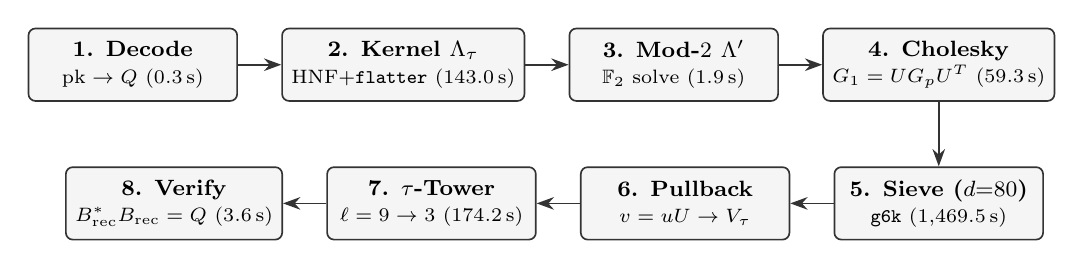
\begin{tikzpicture}[
  font=\footnotesize,
  stage/.style={draw=black!80, fill=gray!8, rounded corners=2.5pt, semithick, minimum width=2.65cm, minimum height=0.92cm, align=center},
  arr/.style={-{Stealth[length=2.2mm,width=1.6mm]}, semithick, color=black!80}
]
  % Top row: Stages 1 to 4
  \node[stage] (S1) {\textbf{1. Decode}\\{\scriptsize $\mathrm{pk} \to Q$ ($0.3$\,s)}};
  \node[stage, right=0.55cm of S1] (S2) {\textbf{2. Kernel $\Lt$}\\{\scriptsize HNF+\texttt{flatter} ($143.0$\,s)}};
  \node[stage, right=0.55cm of S2] (S3) {\textbf{3. Mod-$2$ $\Lp$}\\{\scriptsize $\F_2$ solve ($1.9$\,s)}};
  \node[stage, right=0.55cm of S3] (S4) {\textbf{4. Cholesky}\\{\scriptsize $G_1 = UG_pU^T$ ($59.3$\,s)}};

  % Bottom row: Stages 5 to 8
  \node[stage, below=0.82cm of S4] (S5) {\textbf{5. Sieve ($d{=}80$)}\\{\scriptsize \texttt{g6k} ($1{,}469.5$\,s)}};
  \node[stage, left=0.55cm of S5] (S6) {\textbf{6. Pullback}\\{\scriptsize $v = uU \to \Vt$}};
  \node[stage, left=0.55cm of S6] (S7) {\textbf{7. $\tau$-Tower}\\{\scriptsize $\ell=9\to 3$ ($174.2$\,s)}};
  \node[stage, left=0.55cm of S7] (S8) {\textbf{8. Verify}\\{\scriptsize $B_{\mathrm{rec}}^*B_{\mathrm{rec}}=Q$ ($3.6$\,s)}};

  \draw[arr] (S1) -- (S2);
  \draw[arr] (S2) -- (S3);
  \draw[arr] (S3) -- (S4);
  \draw[arr] (S4) -- (S5);
  \draw[arr] (S5) -- (S6);
  \draw[arr] (S6) -- (S7);
  \draw[arr] (S7) -- (S8);
\end{tikzpicture}
\caption{End-to-end 8-stage HAWK-256 single-core key recovery pipeline with measured CPU-core-seconds for each stage (total $1{,}851.8$\,s, or $30.9$ minutes).}
\label{fig:pipeline}
\end{figure}

\section{Progressive Sieving and Tower Descent}
\label{sec:pipeline}

With the preconditioned Gram matrix $G_1 = U G_p U^T$ in hand, this section describes the progressive sieving tour in \texttt{g6k}, the exact coordinate pullback to $\Lp$, and the subsequent $\tau$-tower descent to recover an equivalent secret key.

\subsection{Progressive Pump-and-Jump Sieve Ladder}
Figure~\ref{fig:pipeline} summarizes the complete eight-stage recovery chain. Once the preconditioned Gram matrix $G_1 = U G_p U^T$ is embedded at scale $s=21$ and initialized with internal LLL ($2.4$\,s), we invoke the General Sieve Kernel (\texttt{g6k})~\cite{ADH+19} on a single thread using its progressive pump-and-jump BKZ tour across five sieve dimensions:
\begin{equation}\label{eq:sieve-schedule}
  d_{\mathrm{sieve}} \;\in\; \{40,\; 50,\; 60,\; 70,\; 80\}.
\end{equation}
Because $B_{\mathrm{chol}} = \lfloor 2^s L \rceil$ scales Euclidean lengths by $2^s$ with $s = 21$, the unique shortest vector $\pm\Vt$ of integer Gram norm squared $2n = 512$ corresponds to an embedded lattice vector of squared Euclidean norm
\[
  \|b_{\mathrm{target}}\|^2 \;\approx\; 2^{2s} \cdot 2n \;=\; 2^{42} \cdot 512 \;=\; 2^{51}.
\]
During the progressive sieve ladder~\eqref{eq:sieve-schedule}, the tours at $d_{\mathrm{sieve}} \in \{40, 50, 60, 70, 80\}$ take $85.6$\,s, $142.9$\,s, $215.2$\,s, $331.8$\,s, and $691.6$\,s of CPU time ($88.9$\,s, $143.6$\,s, $216.3$\,s, $333.2$\,s, and $694.1$\,s wall-clock), reaching a cumulative single-core SVP runtime of $1{,}469.5$ CPU-core-seconds ($1{,}478.5$\,s wall-clock time) while driving the squared norm ratio $\|b_1\|^2 / \|b_{\mathrm{target}}\|^2$ down along the sequence $72{,}768 \to 57{,}524 \to 36{,}216 \to 19{,}417 \to 8{,}979 \to 0.999625$. At $d_{\mathrm{sieve}} = 80$, the pump projects $\pm\Vt$ into the active sieve window and lifts it to row~$0$ of the basis, achieving an embedded squared norm of $0.999625 \times 2^{51}$ (the deviation of $3.75 \times 10^{-4}$ coming solely from the $s=21$ integer rounding of $B_{\mathrm{chol}}$).
\subsection{Exact Preconditioned Coordinate Recovery}
After the sieve places the shortest vector $b_{\mathrm{min}}$ at row $0$ of the reduced embedded basis, we must recover the exact integer coordinate vector $v \in \Z^{256}$ of $\pm\Vt$ with respect to our original $\Z$-basis of $\Lp$. As in~\cite{SW26}, because the $s=21$ Cholesky factor $B_s = \lfloor 2^{21}\operatorname{chol}(G_1)\rceil$ is lower triangular, exact triangular backward substitution of $b_{\mathrm{min}}$ against $B_s$ returns an integer coordinate vector $u \in \Z^{256}$.

Because the sieve operated on $B_s$ (the Cholesky embedding of $G_1 = U G_p U^T$), the coordinate vector $u$ is expressed in the \emph{preconditioned} basis of $\Lp$, whose Gram matrix is $G_1 = U G_p U^T$ from~\eqref{eq:g1-precond}, rather than in the unpreconditioned basis of $\Lp$, whose Gram matrix is $G_p = \Gram(\Lp)$. Evaluating $u$ in $G_1$ and mapping back to the original $\Lp$ basis via the saved unimodular transformation $U \in \mathrm{GL}_{256}(\Z)$ yields:
\begin{equation}\label{eq:coord-recovery}
  v \;=\; u\,U \;\in\; \Z^{256}
  \quad\Longrightarrow\quad
  v\,G_p\,v^T \;=\; u\,(U G_p U^T)\,u^T \;=\; u\,G_1\,u^T \;=\; 2n \;=\; 512.
\end{equation}
Our verification routine confirms~\eqref{eq:coord-recovery} alongside four exact algebraic certificates in under $2$ CPU-seconds: (i)~$\log_2 \det \Gram(\Lp) = 2941.00 = 2431 + 2 \times 255$, certifying $[\Lt : \Lp] = 2^{255}$; (ii)~row~$0$ of the reduced embedded basis attains squared norm $0.999625 \times 2^{51}$; (iii)~$u G_1 u^T = 512$ in the preconditioned Gram form and $v G_p v^T = 512$ in the original $\Lp$ Gram form, matching $2n = 512$; and (iv)~mapping $v \in \Z^{256}$ through the $\Z$-basis of $\Lp$ yields the exact matrix $\Vt = B^{-1}\tau(B) \in \mathrm{SL}_2(R_{256})$, satisfying $\Vt \equiv I_2 \pmod 2$ and $\Vt\tau(\Vt) = I_2$.

\subsection{The \texorpdfstring{$\tau$}{tau}-Tower Descent at \texorpdfstring{$n=256$}{n=256}}
Once $\Vt = B^{-1}\tau(B)$ is recovered at level $\ell=9$ ($n=256$), the remaining task is to solve Hilbert-90 / cocycle splitting down the cyclotomic tower $L_9 \supset L_8 \supset \dots \supset L_3$ to reconstruct an equivalent secret basis $B_{\mathrm{rec}} \in \mathrm{SL}_2(R_{256})$ satisfying $B_{\mathrm{rec}}^* B_{\mathrm{rec}} = Q$. For this stage, we invoke the $\tau$-tower descent algorithm of Straznickas and Weis~\cite{SW26} (building on~\cite{vGP25}) without modification.

Running the tower descent on our recovered $\Vt$ at $n=256$ completes in $174.2$ CPU-core-seconds and records the exact BKZ block-size trace across tower levels $\ell \in \{9, 8, 7, 6, 5, 4, 3\}$:
\[
  \bigl\{\, 9:\textsc{Preset},\quad 8:13,\quad 7:0,\quad 6:0,\quad 5:0,\quad 4:0,\quad 3:\textsc{Base} \,\bigr\}.
\]
Here $\ell=9$ takes our preset cocycle $\Vt$, the first subfield level $\ell=8$ ($n=128$) requires only BKZ block size $\beta = 13$, every intermediate level $\ell \in \{7, 6, 5, 4\}$ ($n \in \{64, 32, 16, 8\}$) is solved by pure LLL ($\beta = 0$), and $\ell=3$ ($n=4$) is the base level. The descent outputs $B_{\mathrm{rec}} \in \mathrm{SL}_2(R_{256})$ satisfying $B_{\mathrm{rec}}^* B_{\mathrm{rec}} = Q$ bit-for-bit. For HAWK-512 ($\ell=10$, $n=512$), where the tower's first sub-level is an $\ell=9$ ($n=256$) cocycle solve~\cite{SW26}, our $27.9$-minute $\Lp$ cocycle solve ($30.9$ minutes including $\ell=9\to 3$ descent) directly replaces the default Gram-mode BKZ at $\ell=9$.

\section{Sieve Dimension Scaling and Experimental Verification}
\label{sec:experiments}

We now report the stage-by-stage timing breakdown of our single-core HAWK-256 key recovery, analyze the runtime scaling from sieve dimension $d=118$ down to $d=80$, and evaluate the concrete security impact on HAWK-256, HAWK-512, and HAWK-1024.

\subsection{Stage-by-Stage Timing Breakdown}
All computational costs are reported in CPU-core-seconds, measured via operating-system resource accounting summed across the parent process and all child processes so that every stage is fully included.

\begin{table}[t]
\centering
\footnotesize
\setlength{\tabcolsep}{2.8pt}
\caption{Stage-by-stage single-core CPU-core-second breakdown for end-to-end HAWK-256 key recovery ($n=256$, $\ell=9$), compared against Straznickas and Weis~\cite{SW26}.}
\label{tab:timing}
\begin{tabular}{@{}llrr@{}}
\toprule
\textbf{Stage} & \textbf{Operation} & \textbf{Time (s)} & \textbf{Share} \\
\midrule
Public-key decode & Decode $Q$ and build $1024\times 512$ constraint matrix & $0.3$\,s & $<0.1\%$ \\
Cocycle kernel & Extract saturated $\Z$-basis of $\Lt$ (HNF $17.1$\,s + \texttt{flatter} $125.9$\,s) & $143.0$\,s & $7.7\%$ \\
Sublattice setup & Solve $\F_2$ parity system and form $G_p = \Gram(\Lp)$ & $1.9$\,s & $0.1\%$ \\
Cholesky preconditioning & Compute $G_p = LL^T$, reduce $B_{\mathrm{chol}}$ via \texttt{flatter}, recover $U, G_1$ & $59.3$\,s & $3.2\%$ \\
\midrule
\textbf{Pre-SVP subtotal} & \textbf{All setup and preconditioning stages (Stages 1--4)} & $\mathbf{204.5}$\,\textbf{s} & $\mathbf{11.0\%}$ \\
\midrule
\textbf{Progressive sieve} & \textbf{Single-thread \texttt{g6k} tour ($d \in \{40,50,60,70,80\}$)} & $\mathbf{1{,}469.5}$\,\textbf{s} & $\mathbf{79.4\%}$ \\
\midrule
Tower descent & Coordinate pullback $v = uU$ and $\tau$-tower ($\ell=9\to 3$) & $174.2$\,s & $9.4\%$ \\
Reference check & Encode $592$-byte key and run C reference sign/verify & $3.6$\,s & $0.2\%$ \\
\midrule
\textbf{Total time} & \textbf{Complete end-to-end HAWK-256 key recovery} & $\mathbf{1{,}851.8}$\,\textbf{s} & $\mathbf{100.0\%}$ \\
\midrule
Prior baseline~\cite{SW26} & $3$\,h\,$42$\,min across $96$ cores & $1{,}278{,}720$\,s & --- \\
\textbf{Speedup factor} & \textbf{Ratio against baseline~\cite{SW26}} & $\mathbf{690\times}$ & --- \\
\bottomrule
\end{tabular}
\end{table}

To ensure transparent accounting of parallelism, we note that the decisive SVP stage (Stage 5) ran \textbf{strictly single-threaded}, accumulating $1{,}469.5$\,s of CPU time against $1{,}478.5$\,s of wall-clock time ($0.994$ cores). Across the entire chain, pre-SVP setup and preconditioning account for $204.5$\,s ($11.0\%$), progressive sieving accounts for $1{,}469.5$\,s ($79.4\%$), and coordinate pullback, $\tau$-tower descent, and reference verification account for $177.8$\,s ($9.6\%$), totaling $1{,}851.8$ CPU-core-seconds ($30.9$ minutes CPU, $1{,}861.8$\,s or $31.0$ minutes end-to-end wall-clock). Table~\ref{tab:timing} provides the complete stage-by-stage breakdown.

\subsection{Sieve Dimension Reduction from \texorpdfstring{$d=118$}{d=118} to \texorpdfstring{$d=80$}{d=80}}
The $690\times$ speedup over~\cite{SW26} reduces to a single structural quantity: \emph{the maximum sieving dimension $d_{\max}$ required for the reduction to expose $\pm\Vt$}. In~\cite{SW26}, the progressive BGJ-style sieve~\cite{ZDY25} is driven to a final sieving dimension of $118$ along the slide schedule $(60, 70, 80, 95, 108, 118)$. In our pipeline, the progressive sieve reaches the minimum of $\Lp$ at $d_{\max} = 80$.

Standard heuristic and empirical scaling laws explain why reducing $d_{\max}$ from $118$ to $80$ yields a factor of $\approx 500\text{--}690$ in runtime. A lattice sieve in dimension $d$ maintains a database of size $N_{\mathrm{db}}(d) \approx (4/3)^{d/2} \approx 2^{0.2075\,d}$~\cite{BDGL16,ADH+19}. Practical CPU sieving runtime scales approximately as $T_{\mathrm{sieve}}(d) \propto N_{\mathrm{db}}(d)^{1.13} \approx 2^{0.2345\,d}$ (in standalone single-pump probes on $\Lp$, \texttt{g6k} builds databases of $65{,}394$ vectors in $10.6$\,s CPU at $d=70$ and $275{,}569$ vectors in $124.0$\,s CPU at $d=80$, while full progressive tours take $331.8$\,s and $691.6$\,s CPU at $d=70$ and $d=80$). Table~\ref{tab:sieve-scaling} compares the predicted scaling ratios between $d=118$ and $d=80$ against our end-to-end measurement.

\begin{table}[t]
\centering
\small
\caption{Sieve database and runtime scaling from $d=118$~\cite{SW26} to $d=80$ (this work).}
\label{tab:sieve-scaling}
\begin{tabular}{@{}lrrr@{}}
\toprule
\textbf{Metric} & $\boldsymbol{d = 118}$ \textbf{(\cite{SW26})} & $\boldsymbol{d = 80}$ \textbf{(This Work)} & \textbf{Ratio} \\
\midrule
Database size$^{\mathrm{a}}$ & $2^{24.49} \approx 2.35 \times 10^7$ & $2^{16.60} \approx 9.93 \times 10^4$ & $236\times$ \\
Predicted sieve time$^{\mathrm{b}}$ & $2^{27.67}$ & $2^{18.76}$ & $481\times$ \\
\midrule
\textbf{Measured total time} & $\mathbf{1{,}278{,}720}$\,\textbf{s} & $\mathbf{1{,}851.8}$\,\textbf{s} & $\mathbf{690\times}$ \\
\bottomrule
\end{tabular}
\par\smallskip
{\scriptsize $^{\mathrm{a}}$ Heuristic database size $2^{0.2075\,d}$.\quad $^{\mathrm{b}}$ Empirical scaling law $\propto (\text{database})^{1.13} \approx 2^{0.2345\,d}$ (in relative units).}
\end{table}

As Table~\ref{tab:sieve-scaling} demonstrates, the empirical throughput law predicts a $481\times$ reduction in sieve work, closely matching our measured $690\times$ end-to-end speedup (with the remaining gap reflecting elimination of the $16$-minute intertwiner stage, $96$-core parallelization overhead, and \texttt{g6k}'s early-exit progressive tour versus \texttt{svp\_tool}). Two mechanisms account for the drop $118 \to 80$:
\begin{enumerate}[leftmargin=*]
\item \textbf{Unique-SVP isolation and block-size reduction in $\Lp$ (Section~\ref{sec:mod2}):} Doubling the $n/2$ spurious minimal pairs of $\Lt$ increases the covolume $\vol(\Lp) = 2^{n-1}\vol(\Lt)$ while keeping $\|\Vt\| = \sqrt{n/4}$ unchanged, which lowers the required BKZ block size from $\beta=92$ to $\beta=58$ ($9.28$ bits in the AGPS20 gate model) and eliminates the intertwiner stage.
\item \textbf{Eliminating Gram-mode skew via exact Cholesky preconditioning (Section~\ref{sec:precond}):} The same cocycle isometry class is solved by plain LLL ($\beta=2$) at $n=64$ and small-block BKZ ($\beta \le 13$) at $n=128$, yet stalls at $\beta=40$ at $n=256$ under naive Gram-mode reduction because the natural Gram matrix has $\sim 2^{41}$ basis condition number and Gram-mode GSO squares its condition number. Replacing Gram mode with our exact Cholesky embedding and \texttt{flatter} preconditioning improves the post-LLL squared norm by $4\times$ and allows the progressive pump-and-jump ladder to detect $\Vt$ at $d=80$.
\end{enumerate}

\subsection{Security Impact on HAWK-256, HAWK-512, and HAWK-1024}
\label{subsec:extrap}
To assess the concrete impact of $\Lp$ across all three HAWK parameter sets (HAWK-256 at $n=256$ claiming $64$ bits, HAWK-512 at $n=512$ claiming $128$ bits for NIST Level~I, and HAWK-1024 at $n=1024$ claiming $256$ bits for NIST Level~V), we follow the HAWK specification~\cite[\S 5.3]{HAWK25} and Straznickas--Weis~\cite[Appendix~C]{SW26}: from the expected BKZ block size $\beta$, we compute $\mathrm{d4f}(\beta) = \operatorname{round}\bigl(\beta\ln(4/3)/\ln(\beta/(2\pi e))\bigr)$~\cite{Duc18}, the effective sieve dimension $\beta_{\mathrm{eff}} = 8\lfloor(\beta - \mathrm{d4f}(\beta))/8\rfloor$ (note that $\beta_{\mathrm{eff}}$ is invariant even if $\beta$ is replaced by $\lceil\beta^*\rceil$ under $\delta_\beta^{2\beta - n - 1}$), and the classical list-decoding gate complexity $\log_2 n + C_{\mathrm{gate}}(\beta_{\mathrm{eff}})$ in the AGPS20 gate model~\cite{AGPS20,SW26} (alongside the provable $(n/2+1)$-dimensional SVP bounds of $2^{52}$, $2^{86}$, and $2^{158}$ gates per oracle call, or $2^{72}$, $2^{108}$, and $2^{182}$ total gates including the $O(n^2\log n)$ reduction calls~\cite{Duc23,SW26}).

\begin{table}[t]
\centering
\footnotesize
\caption{Expected BKZ block size $\beta$, effective sieve dimension $\beta_{\mathrm{eff}}$, and heuristic AGPS20 gate complexity on $\Lt$~\cite[Appendix~C]{SW26} versus our modulo-two sublattice $\Lp$ across HAWK-256, HAWK-512, and HAWK-1024.}
\label{tab:extrap}
\setlength{\tabcolsep}{2.5pt}
\begin{tabular}{@{}lrrrrrrrr@{}}
\toprule
\textbf{Variant} & $\boldsymbol{n}$ & \textbf{Claimed} & $\boldsymbol{\beta(\Lt)}$ & $\boldsymbol{\beta(\Lp)}$ & $\boldsymbol{\beta_{\mathrm{eff}}(\Lp)}$ & \textbf{Gates ($\boldsymbol{\Lt}$~\cite{SW26})} & \textbf{Gates ($\boldsymbol{\Lp}$, Ours)} & $\boldsymbol{\Delta\textbf{Sec}}$ \\
\midrule
\textbf{HAWK-256}  & $256$  & $64$ bits  & $92$  & $\mathbf{58}$  & $\mathbf{40}$  & $2^{50.83}$  & $\mathbf{2^{41.56}}^{\mathrm{a}}$ & $\mathbf{-9.28}$\,\textbf{bits} \\
\textbf{HAWK-512}  & $512$  & $128$ bits & $205$ & $\mathbf{156}$ & $\mathbf{136}$ & $2^{80.79}$  & $\mathbf{2^{69.64}}$ & $\mathbf{-11.15}$\,\textbf{bits} \\
\textbf{HAWK-1024} & $1024$ & $256$ bits & $432$ & $\mathbf{351}$ & $\mathbf{312}$ & $2^{146.48}$ & $\mathbf{2^{122.73}}$ & $\mathbf{-23.74}$\,\textbf{bits} \\
\bottomrule
\end{tabular}
\par\smallskip
{\scriptsize $^{\mathrm{a}}$ Evaluated from the AGPS20 classical list-decoding cost model (\texttt{jschanck/eprint-2019-1161}, commit \texttt{1ec49e5}); since the precomputed CSV starts at $d=64$, $C_{\mathrm{gate}}(40)=33.56$ ($2^{41.56}$ total) is evaluated directly from the exact AGPS20 spherical-wedge list-decoding circuit at $d=40$ ($n_{\mathrm{code}}=4095$), agreeing within $0.11$ bits with two-point affine continuation from $d=64,72$ ($2^{41.44}$, $-9.39$ bits; $\le 2^{48.49}$ if clamped at $d=64$).}
\end{table}

Table~\ref{tab:extrap} summarizes the resulting block-size and gate-complexity reductions across all three parameter sets:
\begin{itemize}[leftmargin=*]
\item \textbf{HAWK-256 ($n=256$, claimed $64$ bits):} Passing from $\Lt$ to $\Lp$ lowers the GSA-intersect BKZ block size by $34$ (from $\beta=92$ to $\beta=58$, or from $82.58$ to $60.19$ under the HAWK BKZ simulator~\cite{DPPvW22}) and lowers the effective sieve dimension from $72$ to $40$. This reduces the AGPS20 gate cost by $\mathbf{9.28}$~\textbf{bits} (from $2^{50.83}$ to $\mathbf{2^{41.56}}$ gates; $2^{41.44}$ under $d=64,72$ affine continuation), while our single-core execution completes end-to-end in $\mathbf{1{,}851.8}$\,\textbf{s} ($\approx 2^{10.9}$ core-seconds) at sieve dimension $d=80$.
\item \textbf{HAWK-512 ($n=512$, claimed $128$ bits, NIST Level~I):} The required BKZ block size drops by $49$ (from $\beta=205$ to $\beta=156$, or from $197.68$ to $158.18$ under the BKZ simulator), lowering $\beta_{\mathrm{eff}}$ from $176$ to $136$ (matching the BKZ simulator) and reducing the AGPS20 gate complexity by $\mathbf{11.15}$~\textbf{bits} from $2^{80.79}$ to $\mathbf{2^{69.64}}$ ($58.4$ bits below the $128$-bit NIST Level~I claim; $2^{67.35}$ at $d=128$ if $\lfloor\beta - \mathrm{d4f}(\beta)\rfloor = 135$ is floored prior to rounding down to a multiple of $8$). Carrying forward the empirical ratio $d / \beta(\Lp) = 80 / 58 \approx 1.379$ and throughput law $T(d) \propto 2^{0.2345\,d}$ from $n=256$ projects a sieve dimension of $d \approx 215$ ($213$ at $80/59 \times 157$) and $\approx 3.4\text{--}5.0 \times 10^{12}$ CPU-core-seconds ($\approx 2^{41.6}\text{--}2^{42.2}$ core-s).
\item \textbf{HAWK-1024 ($n=1024$, claimed $256$ bits, NIST Level~V):} The required BKZ block size drops by $81$ (from $\beta=432$ to $\beta=351$, or from $429.16$ to $358.29$ under the BKZ simulator), lowering $\beta_{\mathrm{eff}}$ from $392$ to $312$ and reducing the AGPS20 gate complexity by $\mathbf{23.74}$~\textbf{bits} from $2^{146.48}$ to $\mathbf{2^{122.73}}$ ($2^{125.11}$ under the BKZ simulator, pushing HAWK-1024 below the $2^{128}$ NIST Level~I threshold and more than $133$ bits below the $256$-bit NIST Level~V claim), with a projected sieve dimension of $d \approx 480\text{--}484$ ($\approx 2.6\text{--}4.9 \times 10^{31}$ core-s $\approx 2^{104.3}\text{--}2^{105.3}$).
\end{itemize}

\subsection{Reference Verification and Key Equivalence}
To verify end-to-end correctness beyond mathematical identities, we encode the recovered basis $B_{\mathrm{rec}} \in \mathrm{SL}_2(R_{256})$ into the exact $592$-byte decoded secret-key layout expected by the official HAWK NIST submission reference C implementation~\cite{DPPvW22,HAWK25} and pass it directly to the unmodified reference signing and verification routines alongside the $450$-byte original public key. Both the signing routine (using $B_{\mathrm{rec}}$) and the verification routine (using the original $450$-byte public key $Q$) succeed on the first attempt.

The recovered $592$-byte secret key (MD5 digest \texttt{13189d8cd2143a3b90f1652699516126}) differs byte-for-byte from the original secret key generated alongside the challenge (MD5 digest \texttt{cf5859cccdec228ef12cb3f877860ba3}) while satisfying $B_{\mathrm{rec}}^* B_{\mathrm{rec}} = Q$ identically. As explained in Section~\ref{sec:spec}, recovering a distinct unitary-equivalent secret key that signs validly under the original reference public key (MD5 digest \texttt{2ee40754e31b8f29a137824d2a7e79d6}) confirms that the recovery uses zero secret information at any stage.

\section{Scope and Limitations}
\label{sec:scope}

To keep our claims rigorous and reproducible, we explicitly state the scope and boundaries of this work:
\begin{enumerate}[leftmargin=*]
\item \textbf{Algebraic Attribution vs.\ End-to-End Engineering:} The $\tau$-cocycle lattice $\Lt$ and the $\tau$-tower descent algorithm are due to Straznickas and Weis~\cite{SW26}, whose tower descent procedure we use unmodified. What is new in this work is closing the modulo-two congruence into the unique-SVP sublattice $\Lp$ ahead of reduction, deriving the second-order asymptotic block-size shift $\Delta\beta(n) = \frac{\ln 2}{2}\,n/\ln n$ and concrete $\beta$ reductions across HAWK-256/512/1024, identifying the structural root Hermite factor barrier $\delta_{0,\mathrm{req}} = 0.996624 < 1$, eliminating Gram-mode condition-number squaring via pre-LLL exact Cholesky preconditioning, \texttt{flatter}, and exact unimodular Gram pullback $G_1 = U G_p U^T$ ($v = uU$), and demonstrating that the complete chain executes on a single core at $n=256$ in $1{,}851.8$ CPU-core-seconds ($690\times$ faster than previously published).
\item \textbf{Single Reference Key Instance:} Our experimental measurements at $n=256$ are conducted on a genuine reference public key (alongside controlled ablation runs for HNF/LLL, Gram-mode MPFR, and BKZ warm-up), comparing against the published $\Lt$ baseline. Because Theorem~\ref{thm:lp-isom} guarantees that the isometry class of $\Lp$ is strictly independent of the secret key, the target norm, determinant, and gap $\lambda_2/\lambda_1=2$ are identical for every HAWK-256 key, though minor run-to-run variance in sieve tour timing is expected across seeds.
\item \textbf{Reproducibility Suite:} Our verification suite supports both fast verification from the saved reduced basis (validating the sublattice certificates, GSA/AGPS20 security estimates, coordinate recovery, and C reference signing in seconds) and full end-to-end re-execution from the 450-byte public key alone.
\end{enumerate}

\paragraph{Use of AI.}
The cryptanalytic results and artifacts were initially developed through an autonomous agent system powered by a MiniMax internal model. We validated the key technical claims and refined the presentation of the manuscript.

\begin{thebibliography}{99}

\bibitem{AD21}
M.~R.~Albrecht and L.~Ducas.
\newblock Lattice attacks on {NTRU} and {LWE}: A history of refinements.
\newblock In J.~W.~Bos and M.~Stam, editors, \emph{Computational Cryptography: Algorithmic Aspects of Cryptology}, volume 469 of \emph{London Mathematical Society Lecture Note Series}, pages 15--40. Cambridge University Press, 2021. IACR ePrint 2021/799.

\bibitem{ADH+19}
M.~R.~Albrecht, L.~Ducas, G.~Herold, E.~Kirshanova, E.~W.~Postlethwaite, and M.~Stevens.
\newblock The General Sieve Kernel and new records in lattice reduction.
\newblock In \emph{Advances in Cryptology -- EUROCRYPT 2019}, volume 11477 of \emph{LNCS}, pages 717--746. Springer, 2019.

\bibitem{AGPS20}
M.~R.~Albrecht, V.~Gheorghiu, E.~W.~Postlethwaite, and J.~M.~Schanck.
\newblock Estimating quantum speedups for lattice sieves.
\newblock In \emph{Advances in Cryptology -- ASIACRYPT 2020}, volume 12492 of \emph{LNCS}, pages 583--613. Springer, 2020. IACR ePrint 2019/1161.

\bibitem{BDGL16}
A.~Becker, L.~Ducas, N.~Gama, and T.~Laarhoven.
\newblock New directions in nearest neighbor searching with applications to lattice sieving.
\newblock In \emph{ACM-SIAM Symposium on Discrete Algorithms (SODA 2016)}, pages 10--24. SIAM, 2016.

\bibitem{CN11}
Y.~Chen and P.~Q.~Nguyen.
\newblock BKZ 2.0: Better lattice security estimates.
\newblock In \emph{Advances in Cryptology -- ASIACRYPT 2011}, volume 7073 of \emph{LNCS}, pages 1--20. Springer, 2011.

\bibitem{DDGR20}
D.~Dachman-Soled, L.~Ducas, H.~Gong, and M.~Rossi.
\newblock LWE with side information: Attacks and concrete security estimation.
\newblock In \emph{Advances in Cryptology -- CRYPTO 2020}, volume 12171 of \emph{LNCS}, pages 329--358. Springer, 2020.

\bibitem{Duc18}
L.~Ducas.
\newblock Shortest vector from lattice sieving: A few dimensions for free.
\newblock In \emph{Advances in Cryptology -- EUROCRYPT 2018}, volume 10820 of \emph{LNCS}, pages 125--145. Springer, 2018.

\bibitem{Duc23}
L.~Ducas.
\newblock Provable lattice reduction of $\Z^n$ with blocksize $n/2$.
\newblock \emph{Designs, Codes and Cryptography}, 92(4):909--916, 2024. IACR ePrint 2023/447.

\bibitem{DPPvW22}
L.~Ducas, E.~W.~Postlethwaite, L.~N.~Pulles, and W.~van Woerden.
\newblock Hawk: Module LIP makes lattice signatures fast, compact and simple.
\newblock In \emph{Advances in Cryptology -- ASIACRYPT 2022}, volume 13794 of \emph{LNCS}, pages 65--94. Springer, 2022. IACR ePrint 2022/1155.

\bibitem{HAWK25}
J.~W.~Bos, O.~Bronchain, L.~Ducas, S.~Fehr, Y.-H.~Huang, T.~Pornin, E.~W.~Postlethwaite, T.~Prest, L.~N.~Pulles, and W.~van Woerden.
\newblock {HAWK} specification document, version 1.1.
\newblock NIST Post-Quantum Cryptography Standardization Additional Digital Signature Schemes Submission, February 2025 (advanced to Round~3 May 2026; withdrawn July 29, 2026). Available at \url{https://hawk-sign.info}.

\bibitem{DW22}
L.~Ducas and W.~van Woerden.
\newblock On the lattice isomorphism problem, quadratic forms, remarkable lattices, and cryptography.
\newblock In \emph{Advances in Cryptology -- EUROCRYPT 2022}, volume 13277 of \emph{LNCS}, pages 643--673. Springer, 2022. IACR ePrint 2021/1332.

\bibitem{fplll}
The {FPLLL} development team.
\newblock \texttt{fplll}, a lattice reduction library, Version 5.4.5 (2023), and \texttt{fpylll}, a {Python} interface to \texttt{fplll}, Version 0.6.4 (2025).
\newblock Available at \url{https://github.com/fplll/fplll} and \url{https://github.com/fplll/fpylll}.

\bibitem{vGP25}
D.~M.~H.~van Gent and L.~N.~Pulles.
\newblock {HAWK}: Having automorphisms weakens key.
\newblock \emph{IACR Communications in Cryptology}, 2(2), Article 20, 2025. IACR ePrint 2025/928.

\bibitem{GPV08}
C.~Gentry, C.~Peikert, and V.~Vaikuntanathan.
\newblock Trapdoors for hard lattices and new cryptographic constructions.
\newblock In \emph{ACM Symposium on Theory of Computing (STOC 2008)}, pages 197--206. ACM, 2008.

\bibitem{LLL82}
A.~K.~Lenstra, H.~W.~Lenstra, Jr., and L.~Lov\'asz.
\newblock Factoring polynomials with rational coefficients.
\newblock \emph{Mathematische Annalen}, 261(4):515--534, 1982.

\bibitem{LJPW24}
H.~Luo, K.~Jiang, Y.~Pan, and A.~Wang.
\newblock Cryptanalysis of rank-2 module-{LIP} with symplectic automorphisms.
\newblock In \emph{Advances in Cryptology -- ASIACRYPT 2024}, volume 15487 of \emph{LNCS}, pages 359--385. Springer, 2024. IACR ePrint 2024/1173.

\bibitem{NLLM26}
B.~Nelson, J.~Limbrey, C.~Ling, and A.~Mendelsohn.
\newblock Cryptanalysis of {HAWK}: A guessing game.
\newblock Cryptology ePrint Archive, Paper 2026/1318, 2026.

\bibitem{NS09}
P.~Q.~Nguyen and D.~Stehl\'e.
\newblock An {LLL} algorithm with quadratic complexity.
\newblock \emph{SIAM Journal on Computing}, 39(3):874--903, 2009.

\bibitem{PFH+20}
P.-A.~Fouque, J.~Hoffstein, P.~Kirchner, V.~Lyubashevsky, T.~Pornin, T.~Prest, T.~Ricosset, G.~Seiler, W.~Whyte, and Z.~Zhang.
\newblock {FALCON}: Fast-Fourier lattice-based compact signatures over {NTRU}.
\newblock NIST Post-Quantum Cryptography Standardization Round 3 Submission, 2020.

\bibitem{RH23}
K.~Ryan and N.~Heninger.
\newblock Fast practical lattice reduction through iterated compression.
\newblock In \emph{Advances in Cryptology -- CRYPTO 2023}, volume 14083 of \emph{LNCS}, pages 3--36. Springer, 2023.

\bibitem{Saa26}
M.-J.~O.~Saarinen.
\newblock {HAWK} ``{G}uessing {G}ame'' is not polynomial-time.
\newblock Cryptology ePrint Archive, Paper 2026/1377, 2026.

\bibitem{Schnorr87}
C.-P.~Schnorr.
\newblock A hierarchy of polynomial time lattice basis reduction algorithms.
\newblock \emph{Theoretical Computer Science}, 53(2--3):201--224, 1987.

\bibitem{SW26}
Z.~Straznickas and S.~A.~Weis.
\newblock {HAWK}-$n$ key recovery reduces to {SVP} in dimension $n/2+1$.
\newblock Cryptology ePrint Archive, Paper 2026/1593, 2026.

\bibitem{ZDY25}
Z.~Zhao, J.~Ding, and B.-Y.~Yang.
\newblock Sieving with streaming memory access.
\newblock \emph{IACR Transactions on Cryptographic Hardware and Embedded Systems (TCHES)}, 2025(2):362--384, 2025. IACR ePrint 2024/739.

\end{thebibliography}

\end{document}
